\documentclass[12pt,a4paper,UTF8]{ctexart}

\usepackage[margin=2.4cm]{geometry}
\usepackage{amsmath,amssymb,bm}
\usepackage{array}
\usepackage{booktabs}
\usepackage{graphicx}
\usepackage{longtable}
\usepackage{setspace}
\usepackage{tikz}
\usetikzlibrary{decorations.pathreplacing}

\begin{document}

\thispagestyle{empty}
\begin{center}
  \zihao{2} 目录
\end{center}

\vspace{1.5em}
\onehalfspacing

\begin{longtable}{>{\raggedright\arraybackslash}p{0.74\textwidth} >{\raggedleft\arraybackslash}p{0.14\textwidth}}
\endhead

量子力学概要 & 1 \\
量子化学的理论基础 & 8 \\
基组 & 50 \\
Gaussian 的相关知识 & 69 \\
GaussView 的使用与分子结构的构建 & 88 \\
单点能的计算与相关问题 & 97 \\
势能面的相关概念 & 119 \\
几何优化 & 122 \\
过渡态搜索 & 139 \\
IRC 的计算与化学反应相关问题 & 151 \\
势能面扫描 & 164 \\
振动分析与红外、拉曼、VCD、ROA 光谱 & 175 \\
热力学量与能量相关性质的计算 & 201 \\
弱相互作用的计算与相关问题 & 229 \\
溶剂模型与溶剂相关问题 & 253 \\
激发态与电子光谱 Part 1：理论基础 & 278 \\
激发态与电子光谱 Part 2：计算与分析实例 & 307 \\
反应速率常数的计算 & 335 \\
磁相关性质的计算 & 354 \\
（超）极化率的计算 & 369 \\
广义与相对论量子化学初步 & 382 \\
分子力学计算、QM/MM 与 ONIOM 方法 & 393 \\
MOPAC 使用简介 & 412 \\
周期性计算简介 & 416 \\
杂项：外电场、背景电荷、偶极矩与多极矩、超精细耦合、$g$ 张量、光学旋转 & 423 \\
量子化学程序盘点 & 436 \\
\end{longtable}

\clearpage
\section{量子力学概要}

和量子化学无关的量子力学知识一概不讲。

更多内容见：
\begin{itemize}
  \item Levine 的 \textit{Quantum Chemistry} 7ed 前一半，有电子版；
  \item \textit{Introduction to Quantum Mechanics}（2ed, Griffiths），市面有影印版及习题解答。
\end{itemize}

更深入内容见：
\begin{itemize}
  \item \textit{Modern Quantum Mechanics}（Sakurai），市面有影印版。
\end{itemize}

经典力学（classical mechanics）适用于描述宏观粒子。它通过位置和速度来描述粒子的状态，其运动方程是牛顿方程。

微观粒子有明显的量子效应，需要改用量子力学（quantum mechanics, QM）研究。量子力学通过波函数（wavefunction）描述粒子的状态，粒子没有确定的位置，行为表现出波粒二象性，其运动方程是薛定谔方程（Schr\"odinger equation）。

\begin{center}
\begin{tikzpicture}[scale=0.95]
  \draw[->] (0,0) -- (5.8,0) node[right] {位置};
  \draw[->] (0,0) -- (0,2.9) node[above] {波函数值};
  \draw[line width=0.9pt, smooth] plot coordinates {
    (0.3,0.05) (0.8,0.08) (1.3,0.20) (1.8,0.75) (2.2,1.75)
    (2.6,2.35) (3.0,2.05) (3.4,1.15) (3.8,0.42) (4.3,0.10) (5.1,0.03)
  };
\end{tikzpicture}
\end{center}

薛定谔方程（单粒子、一维情形）

\begin{center}
\setlength{\fboxsep}{10pt}
\fbox{$\displaystyle i\hbar \frac{\partial \Psi}{\partial t}
=
-\frac{\hbar^2}{2m}\frac{\partial^2 \Psi}{\partial x^2}
+V\Psi$}
\end{center}

其中，$\Psi(x,t)$ 为波函数，$V(x,t)$ 为外势，$x$ 为坐标，$m$ 为粒子质量，$i$ 为虚数符号，$\hbar$ 为普朗克常数除以 $2\pi$。外势和初始状态确定了，粒子的波函数也就确定了。

Born 对波函数的概率解释：
\[
P(x,t)=|\Psi(x,t)|^2=\Psi(x,t)^*\Psi(x,t)
\]
表示 $t$ 时刻粒子在 $x$ 处出现的概率密度。
\[
\int_a^b |\Psi(x,t)|^2\,dx
\]
表示 $t$ 时刻在 $x=[a,b]$ 区间内粒子出现的总概率。

\begin{center}
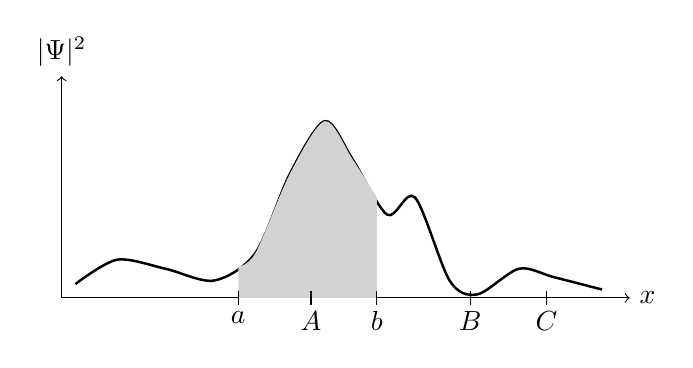
\begin{tikzpicture}[scale=0.88]
  \draw[->] (0,0) -- (8.2,0) node[right] {$x$};
  \draw[->] (0,0) -- (0,3.2) node[above] {$|\Psi|^2$};
  \draw[line width=0.9pt, smooth] plot coordinates {
    (0.2,0.20) (0.8,0.55) (1.5,0.42) (2.2,0.25) (2.8,0.65)
    (3.3,1.80) (3.8,2.55) (4.2,2.00) (4.7,1.20) (5.1,1.45)
    (5.6,0.25) (6.0,0.05) (6.6,0.42) (7.1,0.30) (7.8,0.12)
  };
  \fill[gray!35] (2.55,0) -- plot[smooth] coordinates {
    (2.55,0.45) (2.8,0.65) (3.3,1.80) (3.8,2.55) (4.2,2.00) (4.55,1.45)
  } -- (4.55,0) -- cycle;
  \draw (2.55,-0.10) -- (2.55,0.10) node[below=4pt] {$a$};
  \draw (4.55,-0.10) -- (4.55,0.10) node[below=4pt] {$b$};
  \draw (3.6,-0.10) -- (3.6,0.10) node[below=4pt] {$A$};
  \draw (5.9,-0.10) -- (5.9,0.10) node[below=4pt] {$B$};
  \draw (7.0,-0.10) -- (7.0,0.10) node[below=4pt] {$C$};
\end{tikzpicture}
\end{center}

有物理意义的波函数必须满足归一化条件：
\[
\int_{-\infty}^{+\infty} |\Psi(x,t)|^2\,dx = 1
\]

量子化学中用的波函数一般都是实数型，即
\[
\psi(x)=\psi(x)^*
\]

此时对于单粒子体系，在 $x$ 处出现的概率密度简写为
\[
P(x)=[\psi(x)]^2
\]

当 $V$ 与 $t$ 无关，则体系处于稳态，波函数可写为
\[
\Psi(x,t)=\psi(x)e^{-iEt/\hbar}
\]

对应的概率密度与时间无关，即
\[
|\Psi(x,t)|^2=\Psi^*\Psi=\psi^*e^{iEt/\hbar}\psi e^{-iEt/\hbar}=\psi^*\psi=|\psi(x)|^2
\]

此时薛定谔方程转化为不含时（time-independent）的形式，也称为定态薛定谔方程：

\begin{center}
\setlength{\fboxsep}{10pt}
\fbox{$\displaystyle E\psi=-\frac{\hbar^2}{2m}\frac{d^2\psi}{dx^2}+V\psi$}
\end{center}

其中 $E$ 为体系能量。后面课程涉及的一律为不含时的情况。

算符（operator）用于对它右侧的函数进行某种操作，一般用 $\hat{\ }$（hat）来表明。例如
\[
\hat A=\frac{d}{dx}, \qquad \hat A x^{3/4}=\frac{d\,x^{3/4}}{dx}=\frac{3}{4}x^{-1/4}
\]

算符本身也可以是个函数或常数，例如
\[
\hat A=x, \qquad \hat A x^{3/4}=x^{7/4}
\]

当算符中涉及微分时，和右侧的函数不能互换，即
\[
\hat A f(x)\neq f(x)\hat A
\]

亦不可从等号左右约掉函数，如
\[
\hat A f(x)=C f(x)
\]
不意味着
\[
\hat A=C
\]

对某个函数 $f$ 和常数 $C$，有如下关系时
\[
\hat A f=Cf
\]
$f$ 称为算符 $\hat A$ 的本征函数，$C$ 是其对应的本征值。

对本征函数乘上任意一个常数不会影响它对应的本征值。因此，为了物理意义清楚，一般会给该函数乘以一个因子使之满足归一化条件。

不同的算符对应不同的物理量，不同算符的本征函数集既可以相同也可以不同。

\begin{center}
\renewcommand{\arraystretch}{1.45}
\begin{tabular}{|>{\centering\arraybackslash}p{0.38\textwidth}|>{\centering\arraybackslash}p{0.20\textwidth}|>{\centering\arraybackslash}p{0.16\textwidth}|}
\hline
算符 & 本征函数 & 本征值 \\
\hline
位置算符 $\hat x$ & $\delta(x-x_0)$ & 位置 $x_0$ \\
\hline
动量算符 $\hat p=-i\hbar\dfrac{d}{dx}$ & $e^{ipx/\hbar}$ & 动量 $p$ \\
\hline
动能算符 $\hat T=\dfrac{\hat p\hat p}{2m}=-\dfrac{\hbar^2}{2m}\dfrac{d^2}{dx^2}$ & 同上 & 动能 $p^2/(2m)$ \\
\hline
角动量平方算符 $\hat l^2$ & 球谐函数 & 角动量平方 \\
\hline
哈密顿算符 $\hat H$ & 体系波函数 & 体系能量 \\
\hline
\end{tabular}
\end{center}

位置、动量、动能对应连续谱；角动量平方和体系能量对应离散谱。

如果一个波函数不是某算符的本征函数，那么对此算符对应的属性进行一次观测的话，波函数就会坍塌为此算符的某个本征函数，并且观测到的本征值就是这个本征函数对应的本征值。

例如对一个波函数的位置（对应坐标算符 $\hat x$）进行观测，如果观测到粒子出现在 $x=k$ 的位置，那么波函数就会坍塌为 $\delta(x-k)$。

\begin{center}
\begin{tikzpicture}[scale=0.9]
  \draw[->] (0,0) -- (4.5,0);
  \draw[line width=0.9pt, smooth] plot coordinates {
    (0.3,0.25) (0.9,0.35) (1.5,1.6) (2.0,0.55) (2.5,1.0) (3.0,0.7) (3.6,0.18) (4.1,0.05)
  };
  \draw[->, line width=0.8pt] (5.1,0.9) -- (6.4,0.9);
  \draw[->] (7.0,0) -- (11.0,0);
  \draw[line width=1.0pt] (9.0,0) -- (9.0,2.1);
  \node[below] at (9.0,0) {$k$};
\end{tikzpicture}
\end{center}

哈密顿算符（Hamiltonian operator）包含动能算符 $\hat T$ 和势能算符 $\hat V$ 两部分：
\[
\hat H=\hat T+\hat V
\]

动能算符形式是固定的，如单粒子、一维情形时为
\[
\hat T=-\frac{\hbar^2}{2m}\frac{d^2}{dx^2}
\]

势能算符一般是函数，根据粒子实际所处环境而定。例如，粒子受到中心在原点处的谐振势：
\[
\hat V=\frac{1}{2}kx^2=\frac{1}{2}m\nu^2x^2
\]

电子受到中心在 $x_0$ 处核电荷为 $Z$ 的吸引势：
\[
\hat V=-\frac{Z}{|x-x_0|}
\]

精确求解稳态薛定谔方程 $\hat H\psi=E\psi$ 得到的波函数是 $\hat H$ 的本征函数，本征值是体系能量。此方程往往不止一个解，满足
\[
\hat H \psi_n = E_n \psi_n
\]

能量最低的解称为基态，其余的都是激发态。

若 $E_i=E_j$，则 $i$、$j$ 两个态是能级简并的（degenerate）。

只要有了哈密顿算符的具体形式，原理上就可以求解出体系的波函数，同时得到体系能量，还能进一步求得体系一切其它性质。求解薛定谔方程是量子力学的最关键的问题。

一维谐振子（harmonic oscillator）是最简单的量子力学体系之一，其薛定谔方程为
\[
E\psi=\hat H\psi=\left(-\frac{\hbar^2}{2m}\frac{d^2}{dx^2}+\frac{1}{2}kx^2\right)\psi
\]

对于这样外势函数相对简单的情况可以解析地求解。其能量本征值为
\[
E_n=\left(n+\frac{1}{2}\right)h\nu
\]
其中频率
\[
\nu=\sqrt{k/m}
\]
\[
n=0,1,2,\ldots
\]
$n$ 称为量子数。

其本征函数可写为
\[
\psi_n(x)=\left(\frac{m\nu}{\pi\hbar}\right)^{1/4}\frac{1}{\sqrt{2^n n!}}\,H_n(\xi)e^{-\xi^2/2}
\]
其中
\[
\xi=\sqrt{\frac{m\nu}{\hbar}}\,x
\]

$\{\psi_n\}$ 是 $\hat H$ 的本征函数集合。$n=0$ 对应基态，$n\ge 1$ 对应激发态。

基态时谐振子体系能量不为 $0$，此能量称为零点能（zero point energy, ZPE）：
\[
E_0=\frac{1}{2}h\nu
\]

能解析求解的情况实在太少，大多数定态情况只能通过数值方法近似求解薛定谔方程。

\begin{center}
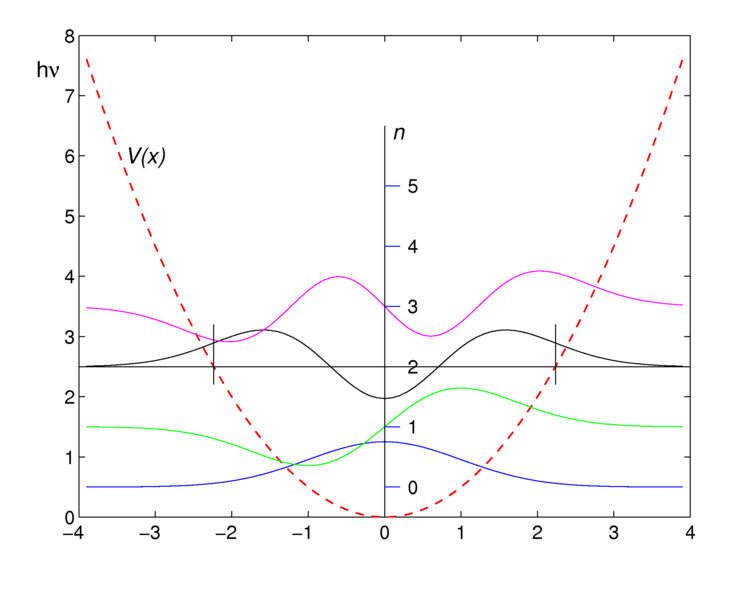
\includegraphics[width=0.47\textwidth]{assets/oscillator_wavefunctions.png}\hfill
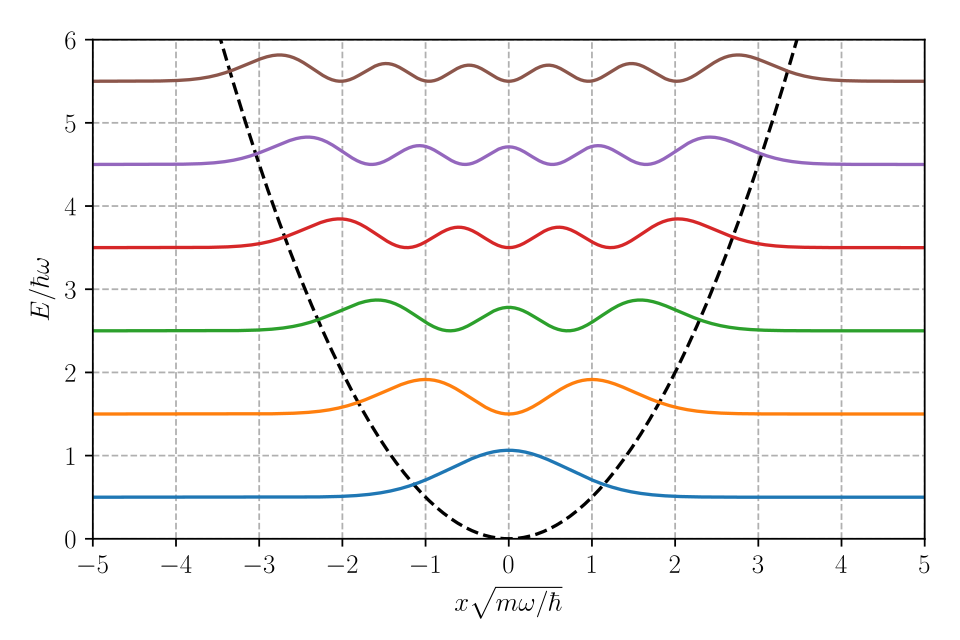
\includegraphics[width=0.47\textwidth,trim=40 30 40 35,clip]{assets/oscillator_probability_densities.png}
\end{center}

如果一个波函数是某个算符的本征函数，那么对此算符相应的属性进行观测，得到的就是其对应的本征值。

如果一个波函数不是某个算符的本征函数，那么每次对它的相应的物理量进行观测可能会得到不同的值。若进行大量观测，所观测到的平均值称为期望值，计算方式为
\[
\langle A\rangle=\int_{-\infty}^{+\infty}\psi(x)^*\,\hat A\,\psi(x)\,dx
\]

例如，实际中粒子的波函数都不是坐标算符的本征函数。若对粒子位置进行大量观测，得到的平均值即为
\[
\langle x\rangle
=
\int_{-\infty}^{+\infty}\psi(x)^*\,x\,\psi(x)\,dx
=
\int_{-\infty}^{+\infty}x\psi(x)^*\psi(x)\,dx
=
\int_{-\infty}^{+\infty}xP(x)\,dx
\]

相当于将坐标乘以相应位置粒子出现概率，然后全空间求和。

当然，若一个波函数本来就是某算符的本征函数，则期望值就是其本征值，如
\[
\langle H\rangle
=
\int_{-\infty}^{+\infty}\psi(x)^*\,\hat H\,\psi(x)\,dx
=
\int_{-\infty}^{+\infty}\psi(x)^*\,E\psi(x)\,dx
\]
\[
=
E\int_{-\infty}^{+\infty}\psi(x)^*\psi(x)\,dx
=
E
\]

有些算符是享有共同的本征函数集的，此时这两个算符间是对易的，即满足
\[
[\hat A,\hat B]=\hat A\hat B-\hat B\hat A=0
\]
即
\[
\hat A\hat B=\hat B\hat A
\]

对易的两个算符对应的两种物理量才是可以同时确定的。例如类氢原子波函数，既是角动量平方算符的本征函数，又是哈密顿算符的本征函数，所以既有确定的角动量平方值，又有确定的能量。

不对易的两个算符对应的两种物理量无法同时确定，如粒子的位置和动量无法同时确定（不确定原理，$\sigma_x\sigma_p\ge \hbar/2$）。

利用狄拉克符号（Dirac notation）不仅可以将量子力学中的积分表达大为简化，对于量子力学理论发展也有特殊意义。

右矢（ket）
\[
|\psi\rangle=\psi(x)
\]

左矢（bra）
\[
\langle \psi|=\int \psi(x)^*[\ldots]\,dx
\]

内积满足
\[
\langle \psi_i|\psi_j\rangle=\int_{-\infty}^{+\infty}\psi_i(x)^*\psi_j(x)\,dx
\]
\[
\langle \psi_i|\psi_j\rangle^*=\langle \psi_j|\psi_i\rangle
\]

算符矩阵元可写为
\[
\langle \psi_i|\hat A|\psi_j\rangle
=
\langle \psi_i|\hat A\psi_j\rangle
=
\int_{-\infty}^{+\infty}\psi_i(x)^*\,\hat A\,\psi_j(x)\,dx
\]

波函数对于某个算符的期望值写作
\[
\langle \psi|\hat A|\psi\rangle
\]

归一化条件
\[
\langle \psi|\psi\rangle=1
\]

正交条件
\[
\langle \psi_i|\psi_j\rangle=0
\]

实际可观测的物理量必定是实数，即
\[
y=y^*
\]

量子力学中，对应于可观测物理量的算符是厄米算符（Hermitian operator）。厄米算符满足
\[
\langle \Psi_i|\hat A\Psi_i\rangle=\langle \hat A\Psi_i|\Psi_i\rangle
\]
即
\[
\int \Psi_i(\mathbf r)^*\,\hat A\,\Psi_i(\mathbf r)\,d\mathbf r
=
\int [\hat A\Psi_i(\mathbf r)]^*\Psi_i(\mathbf r)\,d\mathbf r
\]

亦可由此推得更广义的关系
\[
\langle \Psi_i|\hat A|\Psi_j\rangle
\equiv
\langle \hat A\Psi_i|\Psi_j\rangle
=
\langle \Psi_j|\hat A\Psi_i\rangle^*
\equiv
\langle \Psi_j|\hat A|\Psi_i\rangle^*
\]

动量算符、动能算符、势能算符、哈密顿算符等都是厄米算符。

厄米算符的拥有不同本征值的本征函数彼此间是正交的，具有相同本征值的本征函数（简并态）可以正交也可以不正交，不正交的时候也可以通过对它们线性组合得到彼此正交的本征函数。

例如，量子化学 HF 方法计算产生的分子轨道是 Fock 算符（一种单电子哈密顿算符）的本征函数，本征值是分子轨道能量，故能量不同的分子轨道间必定是正交的。

多电子原子体系无法精确求解薛定谔方程。但是如果只有一个原子核和一个电子，即类氢原子体系，是可以精确求解的，解得的波函数称为原子轨道。

\[
\hat H=-\frac{\hbar^2}{2m_e}\nabla^2-\frac{Ze^2}{4\pi\varepsilon_0 r}
\]

其中 $e$ 为 elementary charge，即质子所带电量，$Z$ 为核电荷数。

求解时需要通过分离变量，将径向和角度部分分离独立求解。

对多电子原子体系，若将电子间相互作用以平均场方式近似考虑，还是可以求解得到原子轨道的，显然结果和类氢原子轨道有一定差异。

原子轨道波函数可写为
\[
\psi_{nlm}\equiv R_{nl}(r)Y_{lm}(\theta,\varphi)
\]
其中 $R_{nl}(r)$ 是径向部分，$Y_{lm}(\theta,\varphi)$ 是角度部分（球谐函数）。

主量子数
\[
n=1,2,3,\ldots
\]

角量子数
\[
l=0,1,2,\ldots,n-1
\]
共 $n$ 个。

磁量子数
\[
m=-l,-l+1,\ldots,0,\ldots,l-1,l
\]
共 $2l+1$ 个。

对于类氢原子，$n$ 决定轨道能量：
\[
E_n=-\frac{Z^2}{2n^2}\ \text{Hartree}
\]

对于多电子原子，$n$ 和 $l$ 共同决定轨道能量。无外磁场时，每个 $(n,l)$ 壳层的 $2l+1$ 个不同磁量子数的轨道能量简并；而有外磁场时，由于 $2l+1$ 个轨道与磁场相互作用能不同，能量将发生分裂。

求解原子的薛定谔方程得到的原子轨道是角动量 $z$ 分量算符 $\hat L_z$ 的本征函数，有的是实函数，有的是复函数，后者不好进行描述和利用。由于每个壳层 $2l+1$ 个轨道能量简并，可以将它们适当线性组合产生出实数型原子轨道波函数，且能量不变。

\[
l=0
\]
称 $s$ 轨道，磁量子数仅为 $0$，只有 $1$ 个轨道。

\[
l=1
\]
称 $p$ 轨道，有 $3$ 个磁量子数，可组合出 $p_x$、$p_y$、$p_z$。

\[
l=2
\]
称 $d$ 轨道，有 $5$ 个磁量子数，可组合出 $d_{xy}$、$d_{yz}$、$d_{xz}$、$d_{x^2-y^2}$、$d_{z^2}$。

\[
l=3
\]
称 $f$ 轨道，有 $7$ 个磁量子数，可组合出 $7$ 个实数型轨道。

在线观看原子轨道图形的程序：$n$ 最高到 $12$，$l$ 最高到 $11$。
\[
\texttt{https://al2me6.github.io/evanescence/}
\]

原子轨道在径向上有 $n-l-1$ 个节点，相应地在径向分布函数上有 $n-l-1$ 个极小点。

\[
1s,\ \text{即 } n=1,\ l=0
\]
\[
2s,\ \text{即 } n=2,\ l=0
\]
\[
2p,\ \text{即 } n=2,\ l=1
\]

实数型原子轨道的角度部分常见为 $s$ 轨道、$p$ 轨道、$d$ 轨道和 $f$ 轨道。

三维、多粒子体系的哈密顿算符可写为
\[
\hat H
=
\sum_i^N\left[-\frac{\hbar^2}{2m_i}\nabla_i^2+V_i(\mathbf r_i)\right]
+
\sum_{i>j}^N V_{ij}(\mathbf r_i,\mathbf r_j)
\]

其中拉普拉斯算符
\[
\nabla_i^2=\frac{d^2}{dx_i^2}+\frac{d^2}{dy_i^2}+\frac{d^2}{dz_i^2}
\]

对应的薛定谔方程为
\[
\hat H\Psi(\mathbf r_1,\mathbf r_2,\ldots,\mathbf r_N)
=
E\Psi(\mathbf r_1,\mathbf r_2,\ldots,\mathbf r_N)
\]

除个别例外，多粒子体系的薛定谔方程从原理上无法解析地求解，只能通过数值方法近似求解。

同时在 $\mathbf r_1'$、$\mathbf r_2'$、$\ldots$、$\mathbf r_N'$ 处都发现一个粒子的概率为
\[
\rho(\mathbf r_1',\mathbf r_2',\cdots,\mathbf r_N')
=
\left|\Psi(\mathbf r_1',\mathbf r_2',\cdots,\mathbf r_N')\right|^2
\]

其归一化条件为
\[
\idotsint \rho(\mathbf r_1,\mathbf r_2,\ldots,\mathbf r_N)\,d\mathbf r_1\,d\mathbf r_2\cdots d\mathbf r_N=1
\]

在 $\mathbf r_1'$、$\mathbf r_2'$ 处都发现一个粒子的概率，而不管其它位置什么情况，为
\[
\rho(\mathbf r_1',\mathbf r_2')
=
N(N-1)\int\cdots\int
\left|\Psi(\mathbf r_1',\mathbf r_2',\ldots,\mathbf r_N)\right|^2
\,d\mathbf r_3\cdots d\mathbf r_N
\]

在 $\mathbf r_1'$ 处发现一个粒子的概率，即单粒子密度，为
\[
\rho(\mathbf r_1')
=
N\int\cdots\int
\left|\Psi(\mathbf r_1',\mathbf r_2,\ldots,\mathbf r_N)\right|^2
\,d\mathbf r_2\,d\mathbf r_3\cdots d\mathbf r_N
\]

对于一个多粒子体系，如果粒子之间没有相互作用（独立粒子），那么整体的波函数可以写为各个波函数的乘积：
\[
\Psi(\mathbf r_1,\mathbf r_2,\cdots,\mathbf r_N)=\psi(\mathbf r_1)\psi(\mathbf r_2)\cdots\psi(\mathbf r_N)
\]

体系总哈密顿是这些独立粒子哈密顿之和：
\[
\hat h_i\psi_i=\varepsilon_i\psi_i
\]
\[
\hat H=\sum_i \hat h_i
\]

体系总能量也是独立粒子能量之和：
\[
E=\sum_i \varepsilon_i
\]

分子体系的电子哈密顿算符中，一般不考虑原子核的量子效应，而把原子核视为有确定位置 $\mathbf R$ 的点电荷。只把电子以量子力学方式考虑。电子的哈密顿为
\[
\hat H_{\mathrm{ele}}
=
\sum_i\left[
-\frac{\hbar^2}{2m_e}\nabla_i^2
-\sum_A\frac{Z_Ae^2}{4\pi\varepsilon_0 r_{iA}}
\right]
+
\sum_{i>j}\frac{e^2}{4\pi\varepsilon_0 r_{ij}}
\]

其中 $r_{iA}$ 是电子 $i$ 与核 $A$ 的距离，$r_{ij}$ 是电子 $i$ 与电子 $j$ 的距离。

原子单位（a.u.）将 $m_e$、$e$、$\hbar$、库仑常数 $1/(4\pi\varepsilon_0)$ 定义为 $1$，使得公式简化许多：
\[
\hat H_{\mathrm{ele}}
=
\sum_i\left[
-\frac{1}{2}\nabla_i^2
-\sum_A\frac{Z_A}{r_{iA}}
\right]
+
\sum_{i>j}\frac{1}{r_{ij}}
\]

体系总哈密顿可以写为
\[
\hat H_{\mathrm{tot}}=\hat H_{\mathrm{ele}}+\hat V_{NN}
\]

在特定的几何坐标下，体系能量等于电子能量与核互斥势能的加和：
\[
E_{\mathrm{tot}}
=(T_{\mathrm{ele}}+V_{\mathrm{ele}})+V_{NN}
=
E_{\mathrm{ele}}+V_{NN}
\]
\[
=
\langle \psi_{\mathrm{ele}}|\hat H_{\mathrm{ele}}|\psi_{\mathrm{ele}}\rangle
+
\sum_{B>A}\frac{Z_AZ_B}{R_{AB}}
\]

量子化学的通用语言中，“电子能量”就是指上式体系总能量 $E_{\mathrm{tot}}$，而非仅仅 $E_{\mathrm{ele}}$ 这一项。

线性组合（linear combination）

对于一个复杂的函数，可以将它写为一套基函数的线性组合的形式，从而便于描述或求解。选用的基函数应当与被展开的函数有相同的边界条件。

\[
|f\rangle \approx \sum_i c_i |g_i\rangle
\]

如果基函数是彼此正交的，则组合系数 $c_i$ 可以通过令向量做投影来得到：
\[
c_i=\langle g_i|f\rangle
\]

完备集（complete set）

如果有一套基函数能够令某个函数被完美地线性展开，则这套基函数对它来说构成完备集。

厄米算符的所有本征函数可以作为完备集来展开与之具有相同边界条件的任何函数。

谐振子体系哈密顿算符的本征函数可以线性组合起来，用来更精确地描述具有相同边界条件的其它函数。

线性变分法（linear variation method）

实际体系的势函数往往比较复杂，导致薛定谔方程不可能直接求解。一个极有用的近似求解方法是线性变分法。即人为地设定一套数学形式比较简单的基函数，记为 $\{\chi\}$，共 $N$ 个，令体系函数对其线性展开来近似地描述：
\[
\Psi \approx \sum_{i=1}^N C_i\chi_i
\]

体系能量
\[
E=\langle \Psi|\hat H|\Psi\rangle
\]

令 $E$ 对这些组合系数的偏导为 $0$：
\[
\frac{\partial E}{\partial C_i}=0,\qquad i=1,2,3,\ldots,N
\]

同时通过拉格朗日乘子法约束它满足归一化条件，就可以找到参数空间 $\{C\}$ 的极值点，即薛定谔方程在当前基函数集下的最优的近似解。所得的各个解满足如下条件：
\[
E_{\mathrm{real}}\le E_1\le E_2\le \cdots \le E_N
\]

$E_{\mathrm{real}}$ 为体系真正基态能量。变分法得到的能量不会比它更低，称为变分原理（variation principle）。

由于限于计算量，实际计算时设定的基函数的数目肯定是有限的，因此通过线性变分法得到的只是近似的解，$E_1$ 必高于真实基态能量。基函数给得越多、越合适，解就越精确，$E_1$ 就越接近真实基态能量。当基函数无穷多时（完备集），$E_1=E_{\mathrm{real}}$。

可以证明，如果给定的 $N$ 个基函数是正交归一的，那么对体系能量进行线性变分，等价于求解如下矩阵本征方程：
\[
\mathbf H\mathbf C=\mathbf C\mathbf E
\]

其中
\[
H_{ij}=\langle \chi_i|\hat H|\chi_j\rangle
\]

求解此方程实际上就是将哈密顿矩阵 $\mathbf H$ 对角化，得到系数矩阵 $\mathbf C$ 和能量矩阵 $\mathbf E$。

\[
C_{mn}
\]
矩阵元对应第 $n$ 个解当中第 $m$ 个基函数的组合系数。

\[
\mathbf E
\]
是对角矩阵，$E_i$ 就是体系的第 $i$ 个解的能量。

求解薛定谔方程从原理上来讲并非难事，线性变分法提供了直接可行的求解对策。量子化学之所以理论、算法复杂且种类繁多，一方面在于会牵扯到电子积分计算等复杂数学问题，一方面牵扯到复杂编程问题，还一方面在于人们不断寻求能以更低的计算量达到更好精度的方法。

维里定理（Virial theorem）

对多原子体系，当原子核受力为 $0$ 时，对于精确波函数，或完备基组下完全以变分方式得到的波函数，如 HF、MCSCF 波函数，势能和动能满足如下关系：
\[
2T_{\mathrm{ele}}=-V_{\mathrm{tot}}=-(V_{\mathrm{ele}}+V_{NN})
\]

维里比值理想值：
\[
-\frac{V_{\mathrm{tot}}}{T_{\mathrm{ele}}}=2
\]

体系总能量：
\[
E_{\mathrm{tot}}=T_{\mathrm{ele}}+V_{\mathrm{tot}}=-T_{\mathrm{ele}}=\frac{V_{\mathrm{tot}}}{2}
\]

Hellmann-Feynman 定理

对于实际精确波函数，或完全变分法得到的波函数且用的基函数不依赖于核坐标，$i$ 原子核（坐标为 $R_i$）的受力可简单写为
\[
F_i=-\frac{\partial E}{\partial R_i}
=
\frac{\partial \langle \Psi|\hat H_{\mathrm{tot}}|\Psi\rangle}{\partial R_i}
=
\left\langle \Psi\left|\frac{\partial \hat H_{\mathrm{tot}}}{\partial R_i}\right|\Psi\right\rangle
\]

满足 Hellmann-Feynman 定理的理论方法在计算原子受力时会比较容易，否则还会额外牵扯到波函数对核坐标的导数项。

电子自旋（electron spin）

不考虑旋轨耦合的情况下，电子波函数可以写为空间部分与自旋部分的乘积：
\[
\psi(\mathbf r;\omega)=\varphi(\mathbf r)\sigma(\omega)
\]

其中 $\varphi$ 为空间函数，$\mathbf r$ 为空间坐标；$\sigma$ 为自旋函数，$\omega$ 为自旋坐标。

电子有 $\alpha$ 和 $\beta$ 两种自旋，对应两种自旋函数，彼此正交：
\[
\sigma(\omega)\in
\left\{
\alpha(\omega),\,
\beta(\omega)
\right\}
\]
\[
\langle \sigma_i|\sigma_j\rangle \equiv \int \sigma_i(\omega)\sigma_j(\omega)\,d\omega
\]
\[
\langle \alpha|\alpha\rangle=1,\qquad
\langle \beta|\beta\rangle=1,\qquad
\langle \alpha|\beta\rangle=0
\]

$\alpha$ 和 $\beta$ 电子的自旋量子数 $s$ 都为 $1/2$，但自旋磁量子数 $m_s$ 分别为 $1/2$ 和 $-1/2$：
\[
\sigma\equiv |s,m_s\rangle,\qquad
\alpha\equiv\left|\frac{1}{2},\frac{1}{2}\right\rangle,\qquad
\beta\equiv\left|\frac{1}{2},-\frac{1}{2}\right\rangle
\]

自旋函数是自旋角动量平方算符和自旋角动量在某一方向分量（一般取 $z$）算符的本征函数：
\[
\hat S^2|s,m_s\rangle=s(s+1)|s,m_s\rangle
\]
\[
\hat S_z|s,m_s\rangle=m_s|s,m_s\rangle
\]

对于多电子体系，自旋部分函数是总自旋角动量平方算符和某一方向分量算符的本征函数：
\[
\hat S^2|S,M_S\rangle=S(S+1)|S,M_S\rangle
\]
\[
\hat S_z|S,M_S\rangle=M_S|S,M_S\rangle
\]

体系如果有 $N$ 个 $\alpha$ 电子、$M$ 个 $\beta$ 电子，那么体系总自旋量子数就为
\[
S=\frac{N-M}{2}
\]
并且有 $2S+1$ 个分量，被称为自旋多重度。这些自旋态分别对应
\[
M_S=-S,-S+1,\ldots,S-1,S
\]

没有外加磁场时，$2S+1$ 个自旋态能量是简并的；而当有外加磁场时，由于电子自旋磁矩和磁场的作用不同，$2S+1$ 个自旋态的能量会发生分裂。

全同粒子体系与反对称原理

量子体系中同种粒子组成全同粒子体系。粒子之间彼此不可分辨，比如不能说第 $i$ 个、第 $j$ 个电子。

自然界粒子分为波色子（Boson）和费米子（Fermion）。费米子包括电子、质子、中子、夸克等；波色子包括光子、胶子、介子等。

费米子构成的全同粒子体系的波函数满足反对称原理，即交换两个费米子的坐标会导致波函数符号变号：
\[
\Psi(\mathbf r_1,\cdots,\mathbf r_i,\cdots,\mathbf r_j,\cdots,\mathbf r_N)
=
-\Psi(\mathbf r_1,\cdots,\mathbf r_j,\cdots,\mathbf r_i,\cdots,\mathbf r_N)
\]

对于波色子构成的波函数，这样交换则不会变号。

这也说明两个自旋相同的电子出现在同一个位置时波函数为 $0$，即概率为 $0$，因为只有 $0$ 才等于它的负值。

推论（Pauli 不相容原理）：两个或多个费米子不能同时处在同一个量子态。如果同时处于同一个量子态，那么它们至少也得有一个属性不同。一个分子轨道不能占据两个自旋相同的电子正是这个道理。

\clearpage
\section{量子化学的理论基础}

课外阅读：辨析计算化学中的任务类型和理论方法。
\[
\texttt{http://sobereva.com/680}
\]

\subsection*{提纲}

\begin{itemize}
  \item 0 前言
  \item 1 量子化学常用理论方法简介
  \item 1.1 Hartree-Fock 方法
  \item 1.2 半经验方法
  \item 1.3 后 HF 方法
  \item 1.3.1 组态相互作用（configuration interaction, CI）
  \item 1.3.2 微扰理论（perturbation theory）
  \item 1.3.3 耦合簇方法（coupled-cluster, CC）
  \item 1.3.4 后 HF 方法的对比
  \item 1.4 MCSCF 与多参考方法简介
  \item 1.5 密度泛函理论
  \item 2 动态相关与静态相关
  \item 3 量子化学中的轨道
  \item 4 自旋多重度、壳层与计算形式
  \item 5 其它
\end{itemize}

\subsection*{前言}

量子化学计算的最核心问题之一是求解化学体系的薛定谔方程。由于哈密顿算符过于复杂而不可能精确求解，在实际数值求解中为了降低计算复杂度和耗时，总是用到各种近似，常见的如：

\begin{itemize}
  \item Born-Oppenheimer 近似
  \item 有限基组近似
  \item 单电子近似、电子相关处理上的近似
  \item 非相对论近似
  \item 数值计算精度上的近似
\end{itemize}

量子化学计算精度关键在于理论方法和基组这两部分。理论方法是厨师，基组是厨具，哪样差了结果都不好。应根据计算能力、对精度的要求选择最适宜的理论方法和基组的搭配。

\begin{center}
\begin{tikzpicture}[scale=0.95]
  \draw[->, line width=1pt] (0,0) -- (5.4,0) node[right] {基组质量};
  \draw[->, line width=1pt] (0,0) -- (0,4.6) node[above] {理论方法};
  \draw[->, line width=1pt] (0,0) -- (4.1,3.4);
  \node[below] at (4.5,0) {完备基组};
  \node[below] at (4.5,-0.45) {(CBS)};
  \node[left] at (0,4.0) {精确考虑电};
  \node[left] at (0,3.55) {子相关作用};
  \node[right] at (4.2,3.45) {精确解};
\end{tikzpicture}
\end{center}

若进一步考虑相对论效应，则在“理论方法”和“基组质量”之外还需再加入一个维度。

\subsection*{Born-Oppenheimer 近似}

严格求解分子体系的定态薛定谔方程时，需要将电子和原子核一起按量子力学方式处理：

\begin{center}
\setlength{\fboxsep}{10pt}
\fbox{$\displaystyle
\hat H_{\mathrm{tot}}\Psi_{\mathrm{tot}}(\mathbf R;\mathbf r)
=
E_{\mathrm{tot}}\Psi_{\mathrm{tot}}(\mathbf R;\mathbf r)$}
\end{center}

由于原子核质量远大于电子，核的量子效应通常远小于电子。Born-Oppenheimer 近似（BO 近似）是量子化学计算中关键性的近似。它将核与电子的运动近似分开处理，从而使核波函数与电子波函数可分别求解，计算复杂度大为简化。总波函数写成
\[
\Psi_{\mathrm{tot}}(\mathbf R;\mathbf r)=\Psi_{\mathrm{nuc}}(\mathbf R)\Psi_{\mathrm{ele}}^{(\mathbf R)}(\mathbf r)
\]
的形式。

在 BO 近似下，求解电子波函数时将核位置视为固定参数，因此它也常被称为核不动近似。对每一组核坐标 $\mathbf R$，都可以求得对应的电子能量 $E_{\mathrm{ele}}^{(\mathbf R)}$；这里的电子能量已包含核间互斥能，因此它是 $\mathbf R$ 的函数，并由此定义了势能面。通常量子化学研究中，求解电子定态方程就已经足够：

\begin{center}
\setlength{\fboxsep}{10pt}
\fbox{$\displaystyle
\hat H_{\mathrm{ele}}^{(\mathbf R)}\psi_{\mathrm{ele}}^{(\mathbf R)}(\mathbf r)
=
E_{\mathrm{ele}}^{(\mathbf R)}\psi_{\mathrm{ele}}^{(\mathbf R)}(\mathbf r)$}
\end{center}

如果研究的问题必须以量子力学方式考虑核的运动，例如量子动力学问题，则可先在不同核坐标下计算电子能量，再拟合成解析的势函数 $E_{\mathrm{pot}}(\mathbf R)$，然后求解核的定态方程，得到核波函数以及包含核运动能在内的体系总能量：
\[
\bigl[\hat T_{\mathrm{nuc}}+E_{\mathrm{pot}}(\mathbf R)\bigr]\Psi_{\mathrm{nuc}}(\mathbf R)
=
E_{\mathrm{tot}}\Psi_{\mathrm{nuc}}(\mathbf R)
\]

一种更便宜得多的考虑核运动量子效应的方法是路径积分分子动力学。

相对于直接精确求解核与电子体系，采用 BO 近似来求解核的定态薛定谔方程并得到核波函数及 $E_{\mathrm{tot}}$ 时，相当于引入了以下近似：

\begin{enumerate}
  \item 绝热近似，即只考虑单个电子态。这相当于忽略了非绝热耦合矩阵（non-adiabatic coupling matrix, NACM）的非对角元；这些项描述不同电子态之间电子与核运动的耦合。
  \item 忽略对角校正项（diagonal correction），即把非绝热耦合矩阵的对角部分也略去。它用于描述单个电子态与核运动的耦合，数量级通常较小。
  \item 忽略质量极化项（mass polarization），它源自体系质心运动与内部运动无法严格分离。
\end{enumerate}

关于上述内容，可参看 \textit{Introduction to Computational Chemistry} 3ed 第 3.1 节。

对于不涉及两个态间势能面交叉的情况，BO 近似通常是相当合理的近似。电子部分计算误差对体系总能量的影响，往往明显大于 BO 近似本身带来的影响。若希望进一步改进结果，可以在计算结束后再加入 diagonal Born-Oppenheimer correction（DBOC）：
\[
\Delta E_{\mathrm{DBOC}}
=
\sum_A^{\mathrm{atoms}}
\left\langle
\Psi_{\mathrm{ele}}
\middle|
-\frac{1}{2M_A}\nabla_A^2
\middle|
\Psi_{\mathrm{ele}}
\right\rangle
\]

但在具体研究涉及的核运动范围内，若存在势能面交叉，则绝热近似由于忽略了态与态之间电子-核耦合的非对角项，会使 BO 近似下得到的能量不够合理。在研究激发态驰豫、态间跃迁等过程时，也需要用到相应电子态之间的非绝热耦合矩阵非对角元。

\subsection*{实际量化计算时分子体系的哈密顿算符}

在实际量化计算中，分子体系常用的电子哈密顿算符写为
\[
\hat H_{\mathrm{ele}}^{(\mathbf R)}
=
\sum_i
\left[
-\frac{1}{2}\nabla_i^2
-\sum_A \frac{Z_A}{|\mathbf r_i-\mathbf R_A|}
\right]
+
\sum_{i>j}\frac{1}{r_{ij}}
+
\sum_{A>B}\frac{Z_AZ_B}{|\mathbf R_A-\mathbf R_B|}
\]
其中，方括号内是单电子部分，包括电子动能与电子-核吸引势；后两项分别为电子间互斥势和核间互斥势。

\subsection*{电子相关与对密度}

电子间相互作用能也可以通过对密度来表示，这样物理图像更易于理解：
\[
E_{ee}
=
\left\langle
\psi\middle|\sum_{i>j}\frac{1}{r_{ij}}\middle|\psi
\right\rangle
=
\iint \frac{\rho(\mathbf r_1,\mathbf r_2)}{r_{12}}\,d\mathbf r_1\,d\mathbf r_2
\]

对密度可分解为
\[
\rho(\mathbf r_1,\mathbf r_2)
=
\bigl[\rho^{\alpha\alpha}(\mathbf r_1,\mathbf r_2)+\rho^{\beta\beta}(\mathbf r_1,\mathbf r_2)\bigr]
+
\bigl[\rho^{\alpha\beta}(\mathbf r_1,\mathbf r_2)+\rho^{\beta\alpha}(\mathbf r_1,\mathbf r_2)\bigr]
=
\rho^{\uparrow\uparrow}(\mathbf r_1,\mathbf r_2)+\rho^{\uparrow\downarrow}(\mathbf r_1,\mathbf r_2)
\]

其中，自旋相同电子对密度和自旋相反电子对密度分别写为
\[
\rho^{\uparrow\uparrow}(\mathbf r_1,\mathbf r_2)
=
\rho^\uparrow(\mathbf r_1)\rho^\uparrow(\mathbf r_2)
+
\Gamma^{\uparrow\uparrow}(\mathbf r_1,\mathbf r_2)
\]
\[
\rho^{\uparrow\downarrow}(\mathbf r_1,\mathbf r_2)
=
\rho^\uparrow(\mathbf r_1)\rho^\downarrow(\mathbf r_2)
+
\Gamma^{\uparrow\downarrow}(\mathbf r_1,\mathbf r_2)
\]

前一项是将电子近似为独立粒子时的对密度，它对 $E_{ee}$ 对应于电子云间的经典库仑互斥；后一项是交换-相关密度，即电子相关作用对对密度的修正，它会使 $E_{ee}$ 降低。

\[
\Gamma^{\uparrow\uparrow}(\mathbf r_1,\mathbf r_2)
=
\Gamma_C^{\uparrow\uparrow}(\mathbf r_1,\mathbf r_2)
+
\Gamma_X^{\uparrow\uparrow}(\mathbf r_1,\mathbf r_2)
\]
\[
\Gamma^{\uparrow\downarrow}(\mathbf r_1,\mathbf r_2)
=
\Gamma_C^{\uparrow\downarrow}(\mathbf r_1,\mathbf r_2)
\]

交换相关（X, exchange correlation）描述自旋相同电子之间的作用。自旋相同的电子间存在 Pauli 互斥，这显著影响对密度分布，也称费米相关；对体系能量的降低称为交换能 $E_X$。

库仑相关（C, Coulomb correlation）描述电子间库仑互斥对对密度的影响。它会降低电子对在较近距离出现的几率，从而降低电子间互斥能；对体系能量的降低称为库仑相关能 $E_C$。

交换相关作用对能量的影响数量级通常远大于库仑相关作用。因此，交换相关若考虑不合理，计算结果会完全离谱；而库仑相关哪怕不考虑，也往往不至于令结果出现定性错误，但若要达到定量精确，则必须充分考虑。

\subsection*{相关穴}

以 $\mathrm{H_2}$ 为例，若已知一个电子出现在某处，由于交换相关和库仑相关，发现另一个电子的概率会发生改变。根据这两个电子自旋相同还是相反，可将这种效应分为费米穴和库仑穴。

费米穴表现出强离域特征，处处为负，最负值为 $-\rho(\mathbf r)$。这说明费米穴总会降低另一个同自旋电子在各处出现的概率，其全空间积分为 $-1$。

库仑穴在参考点附近很负，而在其余部分较正。这表示库仑互斥使另一个电子不容易出现在离当前电子较近的区域，相应地，在更远区域出现的几率会有所增加；其全空间积分为 $0$。

总相关穴由费米穴和库仑穴共同构成。

\subsection*{电子相关作用示意}

若不考虑电子相关，则两个电子的分布彼此独立；若考虑电子相关，则一个电子附近会形成相关穴，另一个电子更倾向于避开这一局域区域。

\subsection*{平均势场近似的直观类比}

不考虑行星之间相关作用时，各行星的运行轨迹可视为在平均势场中的运动；若考虑相关作用，则其它行星的轨迹会产生瞬时影响，轨道也随之偏离理想圆轨道。

\begin{center}
\begin{minipage}{0.46\textwidth}
\centering
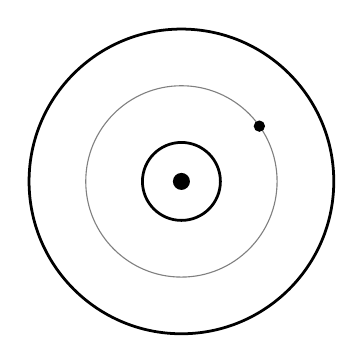
\begin{tikzpicture}[scale=0.9]
  \draw[line width=1pt] (0,0) circle (0.55);
  \draw[gray] (0,0) circle (1.35);
  \draw[line width=1pt] (0,0) circle (2.15);
  \fill (0,0) circle (0.12);
  \fill (1.1,0.78) circle (0.08);
\end{tikzpicture}

不考虑行星之间的相关作用时的运行轨迹，另两个行星的影响以平均势场近似考虑
\end{minipage}
\hfill
\begin{minipage}{0.46\textwidth}
\centering
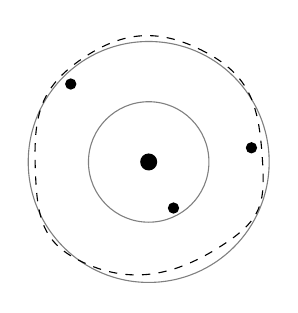
\begin{tikzpicture}[scale=0.9]
  \draw[gray] (0,0) circle (0.85);
  \draw[gray] (0,0) circle (1.7);
  \fill (0,0) circle (0.12);
  \draw[dashed] plot[smooth cycle, tension=0.9] coordinates {(1.6,0.1) (0.8,1.55) (-0.95,1.45) (-1.6,-0.1) (-0.85,-1.45) (1.0,-1.2)};
  \fill (1.45,0.2) circle (0.08);
  \fill (-1.1,1.1) circle (0.08);
  \fill (0.35,-0.65) circle (0.08);
\end{tikzpicture}

考虑行星之间的相关作用时的运行轨迹，其它行星的轨迹产生出瞬时影响
\end{minipage}
\end{center}

\subsection*{1\quad 量子化学常用的理论方法}

常见理论方法可大致分为以下几类：
\begin{itemize}
  \item 半经验方法（semi-empirical），例如 DFTB、GFN-xTB；
  \item 密度泛函理论（density functional theory, DFT）；
  \item Hartree-Fock（HF）；
  \item 后 HF 方法（post-HF），包括微扰理论（perturbation theory）、耦合簇（coupled cluster）、组态相互作用（configuration interaction）、多组态自洽场（MCSCF）以及多参考方法（如 MRCI、CASPT2 等）；
  \item 分子力场方法，它不属于量子化学方法。
\end{itemize}

从头算通常指计算过程中不依赖经验参数的方法，但允许为了加速计算而引入数值近似。至于 DFT 是否严格算作从头算并无必要过分较真。“第一性原理”在字面意义上与从头算相近，但通常包含 DFT，而实际最常用的也正是 DFT。

从精度和花费的粗略排序来看，半经验方法最低，HF 与 DFT 居中，各种形式的后 HF 更高，Full CI 在概念上最为完备。DFT 的计算花费与 HF 相仿，但在描述动态相关方面经验上远优于 HF，因此如今是最常用的方法；HF 单独用于实际研究已经很少见，但它作为后 HF 方法的基础仍然非常重要。

\subsubsection*{1.1\quad Hartree-Fock 方法}

分子体系的哈密顿算符包含多电子间的相互作用，严格求解十分困难。HF 方法将多电子问题转化为单电子问题来处理。它定义了 Fock 算符，使每个电子都看作在其余电子产生的平均势场中运动，这就是单电子近似。

多电子问题满足
\[
\hat H\psi=E\psi
\]
在 HF 近似下，转化为单电子方程
\begin{center}
\setlength{\fboxsep}{10pt}
\fbox{$\displaystyle
\hat F_i\,\varphi_a(\mathbf r_i)=\varepsilon_a\,\varphi_a(\mathbf r_i)$}
\end{center}

其中，$\hat F_i$ 是 Fock 算符，可看作单电子哈密顿算符；$\varphi_a$ 为 HF 轨道，也可视作分子轨道；$\varepsilon_a$ 为 HF 轨道能量。实际计算中，HF 轨道通常通过一套单电子基函数的线性组合来表示，也即 LCAO 形式。

Fock 算符可写为
\[
\hat F_i
=
-\frac{1}{2}\nabla_i^2
-\sum_A \frac{Z_A}{r_{iA}}
+V(\mathbf r_i)
\]
其中，$V(\mathbf r_i)$ 表示其它电子对第 $i$ 个电子产生的平均势场：
\[
V(\mathbf r_i)
=
\int \frac{\rho(\mathbf r')}{|\mathbf r_i-\mathbf r'|}\,d\mathbf r'
+\xi(\mathbf r_i)
\]
前一项是库仑势，来源于经典静电相互作用；后一项是交换势，它来自波函数的反对称要求，纯粹源于量子力学，没有经典物理图像。

因此，HF 使用单电子近似，并不是说某个电子完全不受其它电子影响，而是说它感受到的是其它电子的平均作用。

HF 轨道按能量从低到高填充，遵循 aufbau 原理。最低的 $N$ 个轨道为占据轨道（occupied orbitals），其余为非占据轨道，也称空轨道或虚轨道（virtual orbitals）。

虽然 HF 采用单电子近似，每个电子都视作独立粒子，但体系波函数不能简单写成占据 HF 轨道的直接乘积，因为总波函数必须满足费米子交换反对称要求。因此，HF 波函数必须写成 Slater 行列式形式：
\[
\Psi_{\mathrm{HF}}(\mathbf r_1,\mathbf r_2,\ldots,\mathbf r_N)
=
\frac{1}{\sqrt{N!}}
\begin{vmatrix}
\varphi_1(\mathbf r_1) & \varphi_2(\mathbf r_1) & \cdots & \varphi_N(\mathbf r_1) \\
\varphi_1(\mathbf r_2) & \varphi_2(\mathbf r_2) & \cdots & \varphi_N(\mathbf r_2) \\
\vdots & \vdots & \ddots & \vdots \\
\varphi_1(\mathbf r_N) & \varphi_2(\mathbf r_N) & \cdots & \varphi_N(\mathbf r_N)
\end{vmatrix}
\equiv
\lvert \varphi_1\varphi_2\cdots\varphi_N\rangle
\]

式前的系数是归一化系数。交换任意两个电子坐标，相当于交换行列式中的两行，波函数符号会改变，因此这一形式自动满足反对称要求；若有两个电子占据相同轨道，则行列式为零，也与 Pauli 不相容原理一致。

\subsubsection*{开壳层与闭壳层例子}

以基态 Li 原子 $\left(1s^2\,2s^1\right)$ 为例，它是开壳层体系，包含三个电子，此时波函数可用三个自旋轨道描述：
\[
\Psi(\mathbf r_1,\mathbf r_2,\mathbf r_3)
=
\lvert \varphi_{1s}^{\alpha}\varphi_{1s}^{\beta}\varphi_{2s}^{\alpha}\rangle
=
\frac{1}{\sqrt{6}}
\begin{vmatrix}
\varphi_{1s}^{\alpha}(\mathbf r_1) & \varphi_{1s}^{\beta}(\mathbf r_1) & \varphi_{2s}^{\alpha}(\mathbf r_1) \\
\varphi_{1s}^{\alpha}(\mathbf r_2) & \varphi_{1s}^{\beta}(\mathbf r_2) & \varphi_{2s}^{\alpha}(\mathbf r_2) \\
\varphi_{1s}^{\alpha}(\mathbf r_3) & \varphi_{1s}^{\beta}(\mathbf r_3) & \varphi_{2s}^{\alpha}(\mathbf r_3)
\end{vmatrix}
\]

以基态 Be 原子 $\left(1s^2\,2s^2\right)$ 为例，它是闭壳层体系，包含四个电子。由于电子都是成对的，一对电子可用一个空间轨道描述，因此只需考虑两个空间轨道。对其中一对电子，波函数可写为
\[
\Psi(\mathbf r_1,\mathbf r_2)
=
\lvert \varphi_{1s}\varphi_{2s}\rangle
=
\frac{1}{\sqrt{2}}
\begin{vmatrix}
\varphi_{1s}(\mathbf r_1) & \varphi_{2s}(\mathbf r_1) \\
\varphi_{1s}(\mathbf r_2) & \varphi_{2s}(\mathbf r_2)
\end{vmatrix}
=
\frac{1}{\sqrt{2}}
\bigl[
\varphi_{1s}(\mathbf r_1)\varphi_{2s}(\mathbf r_2)
-\varphi_{2s}(\mathbf r_1)\varphi_{1s}(\mathbf r_2)
\bigr]
\]

若把闭壳层体系按开壳层方式处理，则需要更多自旋轨道，计算耗时更高，但结果完全一样。

\subsubsection*{HF 方法的变分基础}

HF 方程实际上是基于单个 Slater 行列式形式的波函数，通过令体系能量对波函数进行变分并求极小值得到的：
\[
\min \bigl(\langle \Psi_{\mathrm{HF}}\lvert \hat H \rvert \Psi_{\mathrm{HF}}\rangle\bigr)
\]

HF 方法对于 HF 波函数而言，精确考虑了自旋相同电子之间的交换相关作用，因为其 Slater 行列式形式完全满足反对称原理；但由于采用单电子近似，它完全忽略了电子间的库仑相关作用。

由于交换相关作用的重要性和数量级都远大于库仑相关作用，因此 HF 的结果通常仍具有定性正确性；但忽略库仑相关也导致其计算精度不高。

HF 虽然基于单电子近似，但体系总能量并不是所有占据轨道能量的简单加和。每个占据轨道都与其它占据轨道存在经典库仑作用和交换相关作用，若直接相加会把电子间相互作用重复计算一遍，因此在 HF 总能量表达式中需要将这部分扣除。

\subsubsection*{Hartree-Fock-Roothaan 方程}

在实际计算中，HF 方程
\[
\hat F\varphi=\varepsilon\varphi
\]
通常通过 Roothaan 于 1951 年提出的矩阵形式求解，称为 Hartree-Fock-Roothaan（HFR）方程：

\begin{center}
\setlength{\fboxsep}{10pt}
\fbox{$\displaystyle FC=SC\varepsilon$}
\end{center}

其中
\[
F_{\mu\nu}=\langle \chi_\mu \lvert \hat F \rvert \chi_\nu \rangle
\]
\[
S_{\mu\nu}=\langle \chi_\mu \mid \chi_\nu \rangle
\]
\[
\varepsilon_{ii}=\text{轨道能量},\qquad \varepsilon_{i\neq j}=0
\]

若计算时基函数数目为 $N$，则这些矩阵维度均为 $N\times N$，因此求解可得到 $N$ 个轨道。

由于常用基函数一般不是正交的，而是彼此存在重叠，因此出现了重叠矩阵 $S$。$F$ 称为 Fock 矩阵，是 Fock 算符在当前基组下的矩阵表示；$C$ 是系数矩阵，每一列对应一个分子轨道在各个基函数上的展开系数。

实际求解时，先构建 $F$，再通过 Löwdin 正交化消去 $S$，把 Fock 矩阵变为正交基下的 $F'$；随后对 $F'$ 对角化，得到正交基下的本征矢矩阵 $C'$ 和本征值矩阵 $\varepsilon$，最后再逆正交化，将 $C'$ 变换回原基函数下的系数矩阵 $C$。

\subsubsection*{Fock 矩阵、双电子积分与密度矩阵}

HF 计算中最耗时的部分通常是双电子积分，其次是构建 Fock 矩阵。闭壳层情形下，Fock 矩阵元可写为
\[
F_{\mu\nu}
=
\langle \chi_\mu \lvert \hat h \rvert \chi_\nu \rangle
+
\sum_{\lambda\sigma} P_{\lambda\sigma}
\left[
(\mu\nu\vert \sigma\lambda)-\frac{1}{2}(\mu\lambda\vert \sigma\nu)
\right]
\]

其中双电子积分（四指标）定义为
\[
(\mu\nu\vert \sigma\lambda)
=
\iint
\frac{\chi_\mu^*(\mathbf r_1)\chi_\nu^*(\mathbf r_1)\chi_\sigma(\mathbf r_2)\chi_\lambda(\mathbf r_2)}{r_{12}}
\,
d\mathbf r_1\,d\mathbf r_2
\]

密度矩阵可通过轨道系数快速构建，它是对当前体系波函数的一种宏观而紧凑的描述形式。闭壳层形式下，
\[
P_{\lambda\sigma}
=
2\sum_{i=1}^{N_{\mathrm{ele}}/2} C_{\lambda i}C_{\sigma i}^{\mathrm T}
\]

\subsubsection*{单电子算符与单电子积分}

单电子算符定义为
\[
\hat h
=
-\frac{1}{2}\nabla^2
-\sum_A \frac{Z_A}{\lvert \mathbf r-\mathbf R_A\rvert}
\]

单电子积分满足
\[
\langle \chi_\mu \lvert \hat h \rvert \chi_\nu \rangle
=
T_{\mu\nu}
+
\sum_A V_{\mu\nu}^{A}
\]
其中，动能积分为
\[
T_{\mu\nu}
=
-\frac{1}{2}\int \chi_\mu(\mathbf r)\nabla^2\chi_\nu(\mathbf r)\,d\mathbf r
\]
核吸引势积分为
\[
V_{\mu\nu}^{A}
=
-\int \chi_\mu(\mathbf r)\frac{Z_A}{\lvert \mathbf r-\mathbf R_A\rvert}\chi_\nu(\mathbf r)\,d\mathbf r
\]

\subsubsection*{SCF 迭代流程}

HF 方程并不是一步就能直接求解出来。因为构建 Fock 矩阵需要密度矩阵，但密度矩阵在事先又未知，所以基于 HFR 公式计算时，必须先对波函数作一个初始猜测，再由它构造近似的 Fock 矩阵；对角化后得到近似的 HF 能量与波函数，再由该波函数构造更准确的 Fock 矩阵，如此反复，直到体系能量和波函数的变化都很小，任务宣告正常结束。

\begin{center}
\begin{tikzpicture}[x=1cm,y=1cm,>=stealth]
  \tikzstyle{box}=[draw, rectangle, minimum width=3.4cm, minimum height=0.95cm, align=center]
  \node[box] (guess) at (0,0) {初猜波函数};
  \node[box] (fock) at (0,-1.7) {构建 Fock 矩阵};
  \node[box] (diag) at (0,-3.4) {对角化 Fock 矩阵得到\\能量和系数矩阵};
  \node[box] (density) at (0,-5.2) {构建密度矩阵};
  \node[box] (judge) at (0,-6.9) {判断收敛};
  \node[box] (eri) at (4.4,-1.7) {电子积分};
  \node[box] (end) at (5.3,-6.9) {正常结束，输出能量、轨道\\系数等信息};

  \draw[->] (guess) -- (fock);
  \draw[->] (fock) -- (diag);
  \draw[->] (diag) -- (density);
  \draw[->] (density) -- (judge);
  \draw[->] (eri) -- (fock);
  \draw[->] (judge) -- node[above] {已收敛} (end);
  \draw[->] (judge.west) -- ++(-2.0,0) node[midway,below] {未收敛} -- ++(0,5.2) -- (fock.west);
\end{tikzpicture}
\end{center}

HF 方程这种迭代求解的方法也称为自洽场（self-consistent field, SCF）计算。其物理意义相当于
\[
\text{波函数}_0 \rightarrow \text{平均场}_0 \rightarrow \text{波函数}_1 \rightarrow \text{平均场}_1 \rightarrow \cdots
\]
通过迭代不断交替更新波函数与平均场，最终使得在当前波函数所建立的平均场中产生的波函数恰与当前波函数一致。

\begin{center}
\begin{tikzpicture}[x=1cm,y=1cm,>=stealth]
  \node[draw, rounded corners, minimum width=2.3cm, minimum height=0.9cm] (psi) at (0,0.9) {波函数};
  \node[draw, rounded corners, minimum width=2.3cm, minimum height=0.9cm] (field) at (0,-0.9) {平均场};
  \draw[->] (psi.east) .. controls (1.3,0.9) and (1.3,-0.9) .. node[right] {构建} (field.east);
  \draw[->] (field.west) .. controls (-1.3,-0.9) and (-1.3,0.9) .. node[left] {求解} (psi.west);
\end{tikzpicture}
\end{center}

本质上，这也等价于从初猜波函数出发，不断逼近 HF 能量在轨道系数空间中的极小点。对全部占据轨道和基函数而言，在同时施加轨道正交归一约束时，应满足
\[
\frac{\partial E}{\partial C_{\mu i}}=0
\]

\subsubsection*{SCF 收敛与初猜}

SCF 迭代一般在 30 圈以内可以收敛，但在实际问题中，不收敛和难收敛都很常见。可用于辅助收敛的方法很多，例如 DIIS、二次收敛方法（QC）、移位、温度展宽、施加阻尼以及调整初猜等。

大多数程序采用 incremental Fock 方法来加速 SCF 计算，即不是每一轮迭代都根据 Fock 矩阵的公式完整构建它，而是只在上一轮 Fock 矩阵上增量更新。这种方法在弥散函数较多时可能导致难收敛。

产生初猜的方法也很多，例如核哈密顿、扩展休克尔方法、GWH、重叠原子密度（SAD）以及 Harris 泛函等。其中 SAD 的使用最为广泛。

\subsubsection*{SCF 迭代过程中双电子积分的处理}

如果计算中使用了 $N$ 个基函数，则共有约 $N^4/8$ 个双电子积分，因为它们满足八重对称关系：
\[
(\mu\nu\vert \sigma\lambda)
=(\nu\mu\vert \sigma\lambda)
=(\mu\nu\vert \lambda\sigma)
=(\nu\mu\vert \lambda\sigma)
\]
\[
=(\sigma\lambda\vert \mu\nu)
=(\sigma\lambda\vert \nu\mu)
=(\lambda\sigma\vert \mu\nu)
=(\lambda\sigma\vert \nu\mu)
\]

如果内存够大，可以采用 incore 方式做 SCF，即在最初计算一次双电子积分后将其全部保存在内存中，后续各轮 SCF 迭代直接调用。一般情况下，内存并不足以容纳这么多双电子积分；例如用 6-31G$^{**}$ 计算苯需要约 103 MB，而计算卟啉（38 原子）已需要约 21 GB，若基组提升到 def2-TZVP 则需要约 437 GB。

大多数计算采用 direct 方式做 SCF，即在每轮迭代中一边构建 Fock 矩阵元，一边计算所需的双电子积分。它消耗的内存很少，但由于每次迭代都需要把所有双电子积分重新计算一遍，总耗时通常明显高于 incore 方式。不过可以通过积分屏蔽避免计算数值很小的积分，从而有效降低耗时，尤其对大体系更是如此。

conventional 方式和 incore 一样，也是在一开始就把积分算出来备用，但它将积分存到硬盘上。由于硬盘远慢于内存，而现代 CPU 算积分也很快，因此现在 HF 计算里几乎不会再用 conventional 模式，除非是基函数很少的极小体系；而且此模式也非常消耗硬盘，稍大一点体系的所有积分往往根本存不下。

semidirect 是 incore 与 direct 的混合。对于计算代价昂贵的积分，它会存到内存或硬盘中；而每轮迭代时只重新计算便宜的积分，从而在存储空间与计算效率之间取得权衡。支持此模式的程序很少。

\subsubsection*{1.2\quad 半经验方法}

半经验方法是对 Hartree-Fock 方法的近似，主要体现在以下几个方面：
\begin{itemize}
  \item 电子积分通过非常简单的方式近似计算。有些积分被直接忽略，有些则利用许多拟合参数或光谱数据来计算；
  \item 使用极小基，每个原子轨道对应一个 STO 基函数；
  \item 只表现价层原子轨道，忽略内核电子。
\end{itemize}

半经验方法的 SCF 过程和 HF 并无显著区别，但计算耗时通常比 HF 低约两个数量级。处理几十个原子体系很快，处理几百个原子体系也比较轻松，计算上千原子体系往往也没有问题；若利用一些特殊的加速技术，如 MOZYME，甚至可以计算上万个原子体系的能量。

半经验在上世纪 70、80 年代曾是主流。由于计算能力快速提升，从 90 年代后半期开始使用者急剧减少，甚至如今已被很多主流计算工作者遗忘。但它的实用意义仍然显著，例如对体系进行快速初步优化、对大量分子或构型/构象进行快速筛选，以及用于动力学模拟。

主流半经验方法在拟合参数时，基本都是对生成焓进行拟合，因此量化程序输出的其能量，往往对应于标准状况下当前体系的生成焓。

半经验方法由于作了高度近似，在大多数方面的精度和可靠性都逊于 HF，尤其远逊于 DFT；但在计算生成焓时通常优于 HF。一方面是因为生成焓本来就是拟合参数时的目标数据，另一方面也是因为 HF 未考虑的电子相关，在一定程度上被等效吸收到拟合出的参数中。

半经验方法包含针对不同元素的参数，因此不同半经验方法可处理的元素范围并不相同。拟合参数时通常考虑的是成键方式普通的分子，所以半经验方法用于一般有机分子相对稳妥；较新的 PM7 用于配合物和无机材料时，大多也能给出定性正确的结果。但若用于成键方式特殊的体系，则很可能失败。对于一些简单无机分子，半经验方法也可能给出离谱结果，例如 PM7 优化双氧水会得到平面结构。

\subsubsection*{知名的半经验方法}

\begin{itemize}
  \item H\"uckel 分子轨道方法（HMO, 1930）
  \item Pariser-Parr-Pople（PPP, 1953）
  \item 扩展 H\"uckel 方法（EHMO, 1963）
  \item CNDO-1/2（1965/1966）
  \item INDO（1967）
  \item MINDO-1/2/3（1969/1970/1975）
  \item ZINDO（1973/1976）
  \item MNDO（1977）
  \item MNDOC（1981）
  \item AM1（1985）
  \item PM3（1989）
  \item OM1/2/3（1993/2000/2003）
  \item RM1（2006）
  \item PM6（2007）
  \item PM6-DH1、PM6-DH2、PM6-DH+、PM6-DH2X、PM6-D3H4、PM6-D3H4X（2009--2013）
  \item PM7、PM7-TS（2013）
  \item INDO/X（2014）
  \item rPM6（2017）
  \item PM6-D3H4$'$+OH（2023）
\end{itemize}

相关资料：
\[
\texttt{http://sobereva.com/31}
\]
\[
\texttt{http://bbs.keinsci.com/thread-161-1-1.html}
\]

\subsubsection*{代表性研究者与方法}

代表性研究者及其相关方法包括：
\begin{itemize}
  \item Michael J. S. Dewar：MNDO、MINDO、AM1
  \item James J. P. Stewart：PM3、PM6、PM7
  \item John A. Pople：CNDO、INDO
  \item Walter Thiel：MNDO、MNDOC、OM1/2/3
  \item Roald Hoffmann：EHMO
\end{itemize}

\subsubsection*{几种常见半经验方法}

H\"uckel 方法是最古老的半经验方法，由 Erich H\"uckel 于 1930 年提出。它只能用于 $\pi$ 电子体系；扩展 H\"uckel 方法则使其可以用于含 $\sigma$ 电子的体系。该方法非常粗糙，完全忽略了电子-电子互斥项。

AM1（Austin Model 1）和 PM3（Parameterized Model number 3）曾经是最流行的两种半经验方法。凡是支持半经验计算的量化程序，基本都支持它们。二者在不同问题上互有优势，整体水平相近，都不支持过渡金属；后来 PM3 出现过 PM3(TM) 变体，可支持部分过渡金属。如今它们已基本没有实际价值，被 PM6/PM7 完全取代。

PM6 是 PM3 后续发展的第一个公开版本。PM3 之后曾经历 PM4、PM5，但未公开。PM6 除了对 PM3 的精度作出改进、修正其明显缺陷外，支持的元素范围也显著扩大，不仅能处理过渡金属，Bi 之前的元素也都支持。

PM6 计算弱相互作用的精度较差，因此后来出现了多种附加校正版本。Gaussian 中常见的是加入色散校正的 PM6-D3。

\begin{itemize}
  \item PM6-DH1/PM6-DH2：在 PM6 基础上加入色散与氢键校正项；
  \item PM6-DH2X：在 PM6-DH2 的基础上进一步加入对卤键等作用的校正；
  \item PM6-DH+：对弱相互作用的描述比 PM6-DH2 更强，但势能面在一些区域不够平滑；
  \item PM6-D3H+：将 D3 色散和氢键校正同时并入 PM6，整体精度与 PM6-DH+ 相近，GAMESS-US 支持；
  \item PM6-D3H4：除氢键和色散校正外，还加入 Pauli 互斥修正项，MOPAC 支持；
  \item PM6-D3H4X：在 PM6-D3H4 的基础上再加入卤键校正，是 PM6 诸变体中弱相互作用表现最好的方法之一，MOPAC 支持。
\end{itemize}

PM7 是 PM 系列中最新、通常也是最好的一种半经验方法。它通过引入额外修正项，相比 PM6 在弱相互作用描述上有明显改进；但在生成焓等 PM6 传统强项上的提升相对较小。目前支持它的程序主要有 MOPAC 和 Gaussian 16。

PM7-TS 用于过渡态计算时，准确度比 PM6 和 PM7 都有明显改善，但整体误差依然不算理想。

rPM6（reparameterized PM6）是在 PM6 基础上，对某些元素在非限制性开壳层计算情形下重新参数化得到的。对这类体系，它在能量和结构描述上比 PM6 有较大改善；文献测试表明，其 BDE 精度往往强于 PM7，但通常仍逊于 B3LYP。

OM3 在一些文章中被认为是当前算能量较好的半经验方法之一，但由于它长期只在收费且小众的 MNDO 程序中可用，因此实际使用者很少。

TNDO（Typed Neglect of Differential Overlap）是 HyperChem 中用于预测 NMR 的专门半经验方法。

\subsubsection*{1.3\quad 后 HF 方法}

量子化学中通常所说的相关能（correlation energy），定义为后 HF 能量减去 HF 能量：
\[
E_{\mathrm{corr}}=E_{\mathrm{post\text{-}HF}}-E_{\mathrm{HF}}
\]

相关能可以再分为交换相关能和库仑相关能。对于 HF 波函数而言，HF 已经基本合理地描述了自旋相同电子间的交换相关，因为 HF 波函数满足反对称原理；因此后 HF 计算中通常更主要是在补偿 HF 对库仑相关描述不足带来的误差。

需要注意的是：对 HF 波函数本身来说，可以认为 HF 已经较好地刻画了交换相关；但若拿真实精确波函数来比较，尤其在静态相关较强时，也只能说 HF 对交换相关作了基本合理的描述，而不是真正精确。

\begin{center}
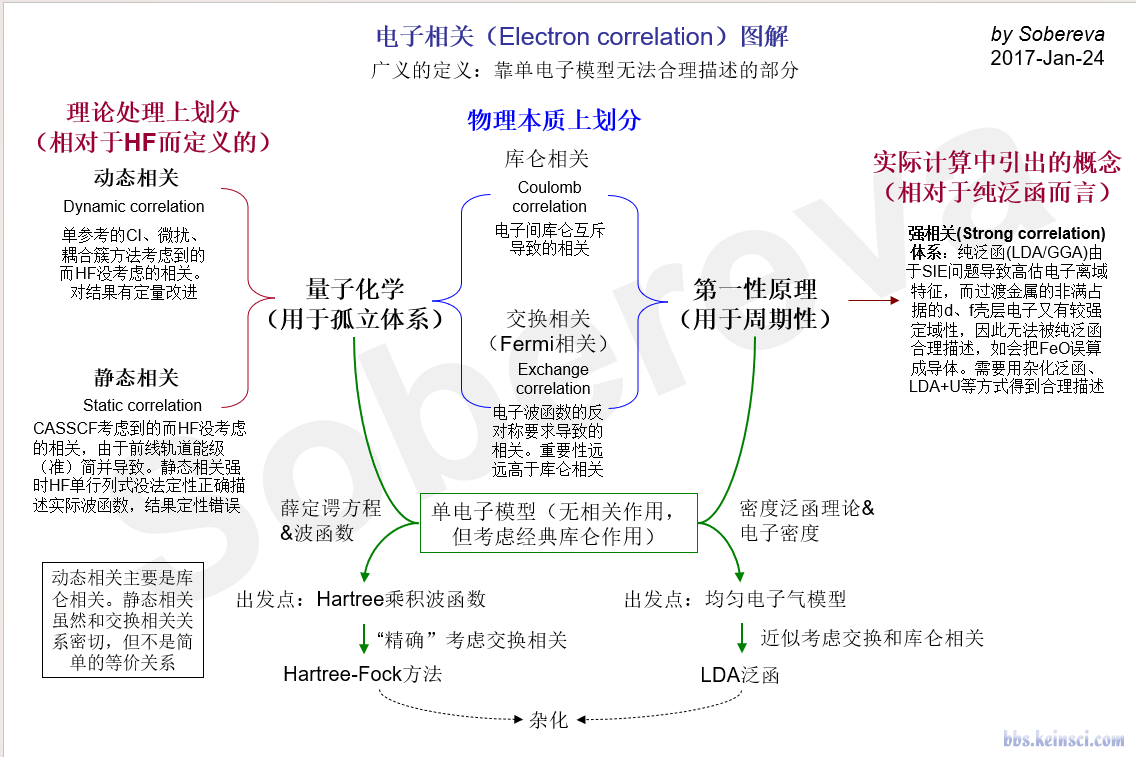
\includegraphics[width=0.72\textwidth]{assets/dianzixiangguan.png}
\end{center}

CI、微扰和耦合簇等方法都属于后 HF（post-HF）方法。它们以 HF 波函数为参考态，进一步计算电子相关能，从而修正 HF 的误差。各种后 HF 方法虽然实现形式不同，但共同点都是不再停留于单电子近似，而是采用大量 Slater 行列式作为多电子基函数来展开真实多电子波函数：
\[
\Psi_m(\mathbf r_1,\mathbf r_2,\cdots,\mathbf r_N)
=
\sum_I c_{I,m}\Phi_I(\mathbf r_1,\mathbf r_2,\cdots,\mathbf r_N)
\]

这些行列式 $\Phi_I$ 可以理解为在 HF 参考波函数的基础上，将占据轨道中的电子以不同方式激发到空轨道后所得到的各种组态。因此，后 HF 方法本质上是用多组态展开来超越单电子近似。

等价地，也可以把这些行列式看作是算符
\[
\sum_i \hat F_i
\]
其中 $i$ 循环所有分子轨道。它们构成的本征函数基可用来展开多电子波函数；其对应本征值则是所占据轨道能量之和。

\begin{center}
\begin{tikzpicture}[x=1cm,y=1cm,>=stealth]
  \tikzstyle{lbl}=[anchor=east]
  \node[lbl] at (-0.4,3.2) {HF 基态波函数};
  \foreach \y in {2.4,1.6,0.8} {
    \draw (0,\y) -- (1.0,\y);
  }
  \draw[->] (0.35,0.8) -- (0.35,1.15);
  \draw[->] (0.65,1.15) -- (0.65,0.8);

  \node[lbl] at (-0.4,-0.1) {各种单激发行列式 $\Phi_i^a$};
  \foreach \x/\up/\down in {2.0/0.8/1.6,3.4/1.6/0.8,4.8/2.4/0.8} {
    \foreach \y in {2.4,1.6,0.8} {
      \draw (\x,\y) -- (\x+1.0,\y);
    }
    \draw[->] (\x+0.35,0.8) -- (\x+0.35,\up+0.35);
    \draw[->] (\x+0.65,\down+0.35) -- (\x+0.65,\down);
  }
  \node at (6.2,1.2) {$\cdots$};

  \node[lbl] at (-0.4,-3.2) {各种双激发行列式 $\Phi_{i,j}^{a,b}$};
  \foreach \x/\a/\b in {2.0/1.6/2.4,3.4/2.4/2.4,4.8/1.6/2.4} {
    \foreach \y in {2.4,1.6,0.8} {
      \draw (\x,\y-3.1) -- (\x+1.0,\y-3.1);
    }
    \draw[->] (\x+0.3,-2.3) -- (\x+0.3,\a-2.75);
    \draw[->] (\x+0.7,-2.3) -- (\x+0.7,\b-2.75);
  }
  \node at (6.2,-2.7) {$\cdots$};
\end{tikzpicture}
\end{center}

HF 波函数就是参考态（reference state）。因此在做后 HF 计算之前，通常都必须先做一次 HF 计算，得到 HF 轨道和参考波函数。

\begin{center}
\begin{tikzpicture}[x=1cm,y=1cm,>=stealth]
  \node[anchor=east] at (-0.2,4.8) {Primitive GTF};
  \node[anchor=east] at (-0.2,3.3) {单电子基函数};
  \node[anchor=east] at (-0.2,1.8) {分子轨道};
  \node[anchor=east] at (-0.2,0.3) {Slater 行列式};
  \node[anchor=east] at (-0.2,-1.6) {比较真实的多电子波函数};

  \node at (2.9,4.8) {$\phi$};
  \node at (2.9,3.3) {$\chi_\mu=\sum_p d_{p,\mu}\phi_p$};
  \node at (2.9,1.8) {$\varphi_i=\sum_\mu C_{\mu i}\chi_\mu$};
  \node at (2.9,0.3) {$\Phi_I=\dfrac{1}{\sqrt{N!}}\lvert\varphi_1\varphi_2\cdots\varphi_N\rangle$};
  \node at (2.9,-1.6) {$\Psi_m=\sum_I C_{I,m}\Phi_I$};

  \draw[->, line width=0.8pt] (2.9,4.35) -- (2.9,3.75);
  \draw[->, line width=0.8pt] (2.9,2.85) -- (2.9,2.25);
  \draw[->, line width=0.8pt] (2.9,1.35) -- (2.9,0.75);
  \draw[->, line width=0.8pt] (2.9,-0.15) -- (2.9,-1.05);

  \node[align=left, anchor=west] at (4.0,3.3) {按照基组的定义收缩};
  \node[align=left, anchor=west] at (4.0,1.8) {``LCAO'' 组合\\（AO 此时指基函数而非原子轨道）};
  \node[align=left, anchor=west] at (4.0,0.3) {反对称乘积};
  \node[align=left, anchor=west] at (4.0,-1.6) {各种方式构造的行列式\\作为多电子基函数展开};

  \draw[decorate,decoration={brace,amplitude=4pt},line width=0.6pt]
    (-1.3,4.95) -- (-1.3,0.0) node[midway,xshift=-0.8cm] {HF};
  \draw[decorate,decoration={brace,amplitude=4pt},line width=0.6pt]
    (-1.3,-0.1) -- (-1.3,-1.95) node[midway,xshift=-0.95cm] {后 HF};
\end{tikzpicture}
\end{center}

\subsubsection*{1.3.1\quad 组态相互作用（configuration interaction, CI）}

CI 方法将真实的多电子波函数写成 HF 波函数以及各种激发行列式或组态态函数（configuration state function, CSF）的线性组合，并通过变分方法求解展开系数，从而得到对应能量。常用的中间归一化写法是令 HF 行列式的系数为 1：
\[
\Psi
=
\Phi_{\mathrm{HF}}
+
\sum_{i,a} c_i^a\Phi_i^a
+
\sum_{\substack{i<j\\a<b}} c_{ij}^{ab}\Phi_{ij}^{ab}
+
\sum_{\substack{i<j<k\\a<b<c}} c_{ijk}^{abc}\Phi_{ijk}^{abc}
+\cdots
\]

这里 $i,j,k$ 代表占据轨道，$a,b,c$ 代表空轨道；$\Phi$ 表示行列式或 CSF。

CI 实际计算中，通常更常用组态态函数（CSF）而不是直接用 Slater 行列式来展开体系波函数，对应的展开系数称为组态系数。

每个 CSF 可以由一个或多个行列式构成。每个 CSF 都是自旋纯态，即它是自旋平方算符 $\hat S^2$ 的本征函数；这也是真实波函数应满足的条件之一。计算时选取的 CSF，其自旋多重度以及自旋磁量子数 $M_S$ 都应与目标态一致。

用 CSF 而非行列式作为多电子基函数来做 CI 的好处，是需要变分的系数往往明显更少；但在做高阶 CI 或 full CI 时，若改用 CSF 表达式，CI 矩阵元会比直接用行列式时复杂得多。

对于无单电子的行列式，它们通常直接对应一个 CSF。对于有单电子的行列式，只有当所有单电子自旋平行时，才直接对应一个 CSF；否则该行列式不是自旋纯态，需要按一定方式作线性组合，才能构成 CSF。

\begin{center}
\begin{tikzpicture}[x=1cm,y=1cm,>=stealth]
  \node[anchor=east] at (0.4,2.7) {自旋纯态，直接作为 CSF};
  \node[anchor=east] at (0.4,0.6) {不对应自旋纯态的行列式};

  \foreach \x/\uone/\utwo in {2.2/0.2/0.9,3.7/0.9/1.6,5.2/0.9/0.2} {
    \draw (\x,2.2) -- (\x+1.0,2.2);
    \draw (\x,2.9) -- (\x+1.0,2.9);
    \draw[->] (\x+0.35,2.2) -- (\x+0.35,2.2+\uone);
    \draw[->] (\x+0.65,2.2) -- (\x+0.65,2.2+\utwo);
  }

  \foreach \x/\up/\down in {2.2/1.6/0.2,3.7/0.9/0.2,5.2/0.2/0.9} {
    \draw (\x,0.1) -- (\x+1.0,0.1);
    \draw (\x,0.8) -- (\x+1.0,0.8);
    \draw[->] (\x+0.35,0.1) -- (\x+0.35,0.1+\up);
    \draw[->] (\x+0.65,0.8) -- (\x+0.65,0.8-\down);
  }
\end{tikzpicture}
\end{center}

若把各阶激发的 CSF 全部都考虑进去，就得到 full CI（FCI）。对于自旋量子数为 $S$、电子数为 $N$、轨道数为 $m$ 的体系，做 full CI 时 CSF 的数目为
\[
N_{\mathrm{CSF}}
=
\frac{2S+1}{m+1}
\binom{m+1}{N/2+S+1}
\binom{m+1}{N/2-S}
\]

若直接用行列式，其数目为
\[
N_{\mathrm{det}}
=
\binom{m}{N_\alpha}\binom{m}{N_\beta}
=
\binom{m}{N/2+S}\binom{m}{N/2-S}
\]

其中组合数满足
\[
\binom{A}{B}=\frac{A!}{(A-B)!\,B!}
\]

由于数目随体系大小迅速爆炸增长，full CI 通常只可能用于非常小的体系和较小的基组。

实际 CI 计算用的都是截断的 CI（truncated CI）。根据所用的 CSF 分为：
\begin{itemize}
  \item CIS：只考虑单重激发 CSF。根据布里渊定理它们与基态 HF 行列式不发生混合，所以只能算激发态。
  \item CID：考虑 HF 波函数及二重激发 CSF。
  \item CISD：考虑 HF 波函数及单重、二重激发 CSF。
  \item CISDT：考虑 HF 波函数及单重、二重、三重激发 CSF。
  \item CISDTQ：考虑 HF 波函数及单重至四重激发 CSF。
  \item CISDTQ5：考虑 HF 波函数及单重至五重激发 CSF。
\end{itemize}

近年来 selected CI（SCI）类型方法开始兴起，可以视为是 FCI 的近似求解。此类方法的共性是通过特定策略快速确定出对能量影响较大的 CSF，只将它们纳入 CI 求解，从而大幅减少了 FCI 要考虑的组态数。虽然比 FCI 可以用于明显更大体系，例如苯分子，但还是超级昂贵，依然是 $N!$ 标度的方法。

CI 计算要求解的方程为
\[
Hc=cE
\]

以 HF 基态波函数 $\lvert 0\rangle$ 和各阶激发态 CSF 为基的哈密顿矩阵 $H$（CI 矩阵）可写为
\begingroup
\setlength{\arraycolsep}{5pt}
\renewcommand{\arraystretch}{1.35}
\[
\resizebox{0.98\textwidth}{!}{$
H=
\left[
\begin{array}{c|cccccc}
 & \Phi_{\mathrm{HF}} & \{\Phi_i^a\} & \{\Phi_{ij}^{ab}\} & \{\Phi_{ijk}^{abc}\} & \{\Phi_{ijkl}^{abcd}\} & \cdots \\
\hline
\Phi_{\mathrm{HF}} & \langle 0|\hat H|0\rangle & 0 & \langle 0|\hat H|D\rangle & 0 & 0 & \cdots \\
\{\Phi_i^a\} & 0 & \langle S|\hat H|S\rangle & \langle S|\hat H|D\rangle & \langle S|\hat H|T\rangle & 0 & \cdots \\
\{\Phi_{ij}^{ab}\} & \langle D|\hat H|0\rangle & \langle D|\hat H|S\rangle & \langle D|\hat H|D\rangle & \langle D|\hat H|T\rangle & \langle D|\hat H|Q\rangle & \cdots \\
\{\Phi_{ijk}^{abc}\} & 0 & \langle T|\hat H|S\rangle & \langle T|\hat H|D\rangle & \langle T|\hat H|T\rangle & \langle T|\hat H|Q\rangle & \cdots \\
\{\Phi_{ijkl}^{abcd}\} & 0 & 0 & \langle Q|\hat H|D\rangle & \langle Q|\hat H|T\rangle & \langle Q|\hat H|Q\rangle & \cdots \\
\vdots & \vdots & \vdots & \vdots & \vdots & \vdots & \ddots
\end{array}
\right]
$}
\]
\endgroup

\[
\text{左下和右上对称}
\]

HF 基态与单激发 CSF 不直接混合是因为布里渊定理，而相对激发数超过 2 的 CSF 不直接混合是因为哈密顿算符只包含单、双电子项。

CI 计算主要耗时的就是构建 $H$ 矩阵，以及之后对 $H$ 对角化得到本征矢矩阵 $c$ 和本征值矩阵 $E$。最低本征值是基态能量，往上依次是第一、第二激发态能量，因此 CI 可以直接求解激发态。$c$ 的每一列对应一个态中的各个 CSF 或行列式的组合系数。

由于 CI 矩阵维度通常很高，特别是高阶 CI 甚至达到上百万、上千万，对角化整个矩阵一般无法做到，所以实际计算中大多都通过 Davidson 迭代方法来求解，相当于把问题转化为在维度较小的子空间中对角化 CI 矩阵，并随着迭代进行以一定方式逐渐扩张子空间维度。当感兴趣的最低的一批解的能量和波函数变化都已经很小时，或以一定方式估计的误差值小于阈值时，迭代结束。

CI 的一个好处是满足变分原理，即得到的能量肯定不会低于真实能量。但这个好处对实际研究一般并不重要。

除 CIS 以外的截断的 CI 方法不满足尺寸一致性（size-consistent）。比如 CISD 计算相距无限远的含有两个氢分子的体系，其能量并不等于两个氢分子的加和。这个问题使得 CI 不可能用于分子间相互作用的计算。而 HF、DFT、微扰、耦合簇方法都满足尺寸一致性。

Davidson 校正是对 CISD 的后处理校正，以免费的方式近似得到考虑四重激发 CSF 后对能量的修正。这对结果精度有改进，并很大程度缓解 CISD 不满足尺寸一致性的问题：
\[
\Delta E_Q \approx (1-c_{\mathrm{HF}}^2)(E_{\mathrm{CISD}}-E_{\mathrm{HF}})
\]
\[
E_{\mathrm{CISD+Q}}=E_{\mathrm{CISD}}+\Delta E_Q
\]
其中 $c_{\mathrm{HF}}$ 是完全归一化后的 CISD 波函数中的 HF 系数。

同样计算量下，CI 的结果不如微扰、耦合簇，因此很不划算，很少被直接使用计算基态性质。

\subsubsection*{1.3.2\quad 微扰理论（perturbation theory）}

如果一个哈密顿太复杂，不好直接求解薛定谔方程，那么可以写为两部分的加和，即比较容易求解的零阶哈密顿加上扰动量：
\[
\hat H=\hat H^0+\hat H'
\]

先用未扰动哈密顿求解薛定谔方程，得到对应的波函数 $\psi_0^{(0)}$ 和能量 $E_0^{(0)}$，然后再把扰动的效果加进去：
\[
E_0=E_0^{(0)}+E_0^{(1)}+E_0^{(2)}+\cdots
\qquad
\psi_0=\psi_0^{(0)}+\psi_0^{(1)}+\psi_0^{(2)}+\cdots
\]

$n$ 阶微扰理论就是考虑到 $n$ 阶修正，下标 0 代表基态：
\[
E_0^{(0)}=\left\langle \psi_0^{(0)} \middle| \hat H^0 \middle| \psi_0^{(0)} \right\rangle
\]
\[
E_0^{(1)}=\left\langle \psi_0^{(0)} \middle| \hat H' \middle| \psi_0^{(0)} \right\rangle
\]
\[
E_0^{(2)}=\left\langle \psi_0^{(0)} \middle| \hat H' \middle| \psi_0^{(1)} \right\rangle
\]
\[
E_0^{(3)}=\left\langle \psi_0^{(0)} \middle| \hat H' \middle| \psi_0^{(2)} \right\rangle
\]

M{\o}ller--Plesset 于 1934 年提出将微扰理论用于分子体系计算的具体形式，将哈密顿划分为
\[
\hat H'=\hat H^{\mathrm{real}}-\hat H^0
=
\left(\sum_i \hat h_i+\sum_{i>j}\frac{1}{r_{ij}}\right)-\sum_i \hat F_i
\]

MP$n$ 表示考虑到 $n$ 阶微扰，如 MP2 就是考虑到 $E^{(2)}$。HF 占据轨道能量之和相当于 0 阶能量，HF 能量实际上是 MP1 能量，因此最低阶微扰计算的是 MP2。

MP2 总能量在实际量化计算中的具体表达式为
\[
E^{\mathrm{MP2}}
=
\underbrace{E^{(0)}+E^{(1)}}_{\text{HF 能量}}
+
\underbrace{E^{(2)}}_{\text{MP2 相关能}}
\]

\[
E^{(0)}
=
\sum_i^{\mathrm{occ}} \varepsilon_i
=
\sum_i^{\mathrm{occ}} \langle i|\hat h|i\rangle
+
\sum_{i,j}^{\mathrm{occ}} \langle ij\Vert ij\rangle
\]

\[
E^{(1)}
=
-\frac{1}{2}\sum_{i,j}^{\mathrm{occ}} \langle ij\Vert ij\rangle
\]
其中 $i,j$ 为单占据自旋轨道。库仑积分为 $J_{ij}$，交换积分为 $K_{ij}$，并且
\[
\langle ij\Vert ij\rangle=
\begin{cases}
(ii|jj)-(ij|ji), & i \text{ 与 } j \text{ 自旋相同} \\
(ii|jj), & i \text{ 与 } j \text{ 自旋相反}
\end{cases}
\]

基态波函数的一阶微扰校正可以写成其它态的 0 阶波函数的线性展开：
\[
\psi_0^{(1)}=\sum_{m\ne 0} c_m\psi_m^{(0)}
\]
\[
c_m=
\frac{\langle \psi_m^{(0)}|\hat H'|\psi_0^{(0)}\rangle}{E_0^{(0)}-E_m^{(0)}}
\]
其中下标 $m$ 表示态的标号。于是 MP2 相关能可写为
\[
E_0^{(2)}
=
\left\langle \psi_0^{(0)} \middle| \hat H' \middle| \psi_0^{(1)} \right\rangle
=
\sum_{m\ne 0}
\frac{\left|\left\langle \psi_0^{(0)} \middle| \hat H' \middle| \psi_m^{(0)} \right\rangle\right|^2}{E_0^{(0)}-E_m^{(0)}}
\]

基态的 0 阶波函数 $\psi_0^{(0)}$ 就是 HF 行列式，其它态的 0 阶波函数 $\psi_m^{(0)}$ 取各种方式激发的行列式，对应的零阶能量就是占据轨道能的加和。可以证明只有双激发行列式才会出现在 MP2 相关能中：
\[
E_0^{(2)}
=
\sum_{i<j}^{\mathrm{occ}}\sum_{a<b}^{\mathrm{vir}}
\frac{
\left|
\left\langle \Phi_{\mathrm{HF}}
\middle|
\sum_{r<s}\frac{1}{r_{rs}}
\middle|
\Phi_{ij}^{ab}
\right\rangle
\right|^2
}{
\varepsilon_i+\varepsilon_j-\varepsilon_a-\varepsilon_b
}
\]
\[
=
\frac{1}{4}\sum_{i,j}^{\mathrm{occ}}\sum_{a,b}^{\mathrm{vir}}
\frac{\left|(ia|jb)-(ib|ja)\right|^2}{\varepsilon_i+\varepsilon_j-\varepsilon_a-\varepsilon_b}
\]
其中 $i,j$ 为单占据自旋轨道，$a,b$ 为非占据自旋轨道，$r,s$ 为电子标号。

MP2--MP6 的最高阶微扰校正项所涉及的耦合层级可概括为：随着阶数提高，最高阶项中逐步出现 HF 基态以及单、二、三、四、五、六重激发行列式之间的耦合。记号中 0 表示 HF 基态行列式，S/D/T/Q/P/H 分别表示单/二/三/四/五/六重激发行列式，$V$ 表示扰动哈密顿算符。

MP$n$ 随着 $n$ 增大，未必结果会顺利收敛，有时可能会震荡、收敛缓慢，或发散。

MP2 是所有后 HF 计算级别中最便宜的一种。计算量不算太大，精度比 HF 改善明显，但用于过渡金属不理想，尤其是开壳层、配位不饱和体系、镧系、锕系、静态相关明显的体系。往往高估键长、略高估过渡态势垒；对第一行过渡金属配合物的金属-配体键长则明显被低估。

在能达到相似或更好精度且计算量低得多的 DFT 流行起来后，MP2 被使用得就越来越少了。不过后来兴起的 SCS-MP2、MP2.5 等变体使得微扰理论又焕发了新的活力。

主流量化程序都支持 MP2，一般最高支持到 MP4。MP3 对 MP2 改进不大，容易低估相关能，时常还不如 MP2，不建议使用。MP5 由于很昂贵而实用性差，且很少有程序支持（但 Gaussian 支持）。如今高精度计算一般用各方面更优秀的耦合簇方法来做，很少靠高阶微扰理论实现。

MP4 有两种常用的具体形式，MP4(SDQ) 和 MP4(SDTQ)。前者把三重激发行列式忽略掉，可以节省大量计算时间，但是精度比 MP4(SDTQ) 也有所下降，例如低估色散作用能。

\subsubsection*{开壳层微扰理论}

微扰理论对于开壳层一般是基于 UHF 波函数做的，即 UMP，结果不算理想，容易有较大自旋污染问题，但通过自旋投影可以改善，称 PUMP 或 PMP（projected MP）。

微扰也可以基于 ROHF 轨道做，有不同具体实现，优缺点也不尽相同。分为两类：
\begin{itemize}
  \item 零阶哈密顿算符与 $S^2$ 算符不对易，有自旋污染，包括 ROMP、RMP、ROHF-MBPT、ZAPT。
  \item 零阶哈密顿算符与 $S^2$ 算符对易，无自旋污染，包括 OPT、IOPT、HCPT、陈飞武的 OSPT。
\end{itemize}

\subsubsection*{MP2 变体}

SCS-MP2（spin-component scaled MP2）将 MP2 相关能分解为自旋平行和自旋反平行两部分：
\[
E^{(2)}=E_{\mathrm{SS}}+E_{\mathrm{OS}}
\]
其中 $E_{\mathrm{SS}}$ 为自旋平行电子对对 MP2 相关能的贡献，即 MP2 相关能表达式里二重激发行列式中两个被激发的电子都是 $\alpha$ 或都是 $\beta$；$E_{\mathrm{OS}}$ 为自旋反平行电子对对 MP2 相关能的贡献，即两个被激发的电子一个是 $\alpha$、另一个是 $\beta$。

由于 HF 已经考虑了很多自旋平行电子的相关作用（交换相关作用），因此 MP2 中应弱化自旋平行部分。SCS-MP2 调整了 MP2 相关能的自旋平行和反平行部分的系数：
\[
E^{(2)}=\frac{1}{3}E_{\mathrm{SS}}+\frac{6}{5}E_{\mathrm{OS}}
\]

SCS-MP2 算反应能号称比 MP2 有了很大提高（实际情况也并非总是如此），几何结构也比 MP2 略有改进，但势垒计算精度比 MP2 反倒略低一点，弱相互作用计算精度恶化不少，其它方面和 MP2 差不多。整体性能明显不如目前最好的双杂化泛函。相关文献为 \textit{J. Chem. Phys.}, 118, 9095 (2003)。

\begin{itemize}
  \item SOS-MP2：忽略了自旋平行贡献，反平行部分乘以 1.3，结果比 MP2 差，特别是弱相互作用。不过通过算法上的优化可以令计算花费比 MP2 低。
  \item GIAO-SCS-MP2：借鉴 SCS-MP2 思路，专门用于计算 NMR，结果接近 CCSD(T)。磁屏蔽张量计算方式为 HF 贡献 $+c_1\times$ MP2 自旋平行贡献 $+c_2\times$ MP2 自旋反平行贡献，$c_1$、$c_2$ 向精确计算结果拟合，且目前没有公开程序支持。
  \item SCS-MP3：SCS-MP2 能量加上乘以 0.25 的 $E^{(3)}$ 校正能。热化学性能比 SCS-MP2 好很多，号称有时接近 QCISD(T)，但低估弱相互作用能。
\end{itemize}

文献中给出了若干方法对反应能和原子化能的统计结果，误差列分别为平均误差、MAE、最大误差以及误差超过 3 kcal/mol 的数目：

\begin{center}
\small
\begin{tabular}{lrrrr}
\toprule
方法 & Mean & MAE & MAX & $N_{>3}$ \\
\midrule
\multicolumn{5}{c}{Reaction energies, $N=32$} \\
QCISD(T) & 0.2 & 0.7 & 4.5 & 1 \\
QCISD & -1.2 & 2.2 & 7.0 & 9 \\
MP2 & -3.1 & 4.1 & 13.9 & 17 \\
MP3 & -3.9 & 4.9 & 25.3 & 23 \\
SCS-MP2 & -0.3 & 1.9 & 5.1 & 6 \\
SCS-MP3 & -0.4 & 1.3 & 3.9 & 1 \\
\midrule
\multicolumn{5}{c}{Atomization energies, $N=11$} \\
QCISD(T) & -0.6 & 0.7 & 2.9 & 0 \\
QCISD & -0.2 & 6.4 & 17.8 & 8 \\
MP2 & 6.2 & 7.9 & 24.6 & 8 \\
MP3 & -7.7 & 7.7 & 33.8 & 8 \\
SCS-MP2 & 5.7 & 5.7 & 15.4 & 6 \\
SCS-MP3 & 1.3 & 2.6 & 9.3 & 4 \\
\bottomrule
\end{tabular}
\normalsize
\end{center}

相关文献为 \textit{J. Comput. Chem.}, 24, 1529 (2003)。

\begin{itemize}
  \item SCS(MI)-MP2：平行、反平行系数来自拟合 S22 弱相互作用测试集。对于 cc-pV$n$Z 系列基组两种都分别拟合了参数。弱相互作用计算误差比 MP2 低两到三倍。
  \item SCSN-MP2：忽略自旋反平行部分，自旋平行部分的系数为 1.76，拟合自核酸碱基对相互作用能。弱相互作用计算精度和 SCS(MI)-MP2 相仿。
  \item SCS-S66-MP2：利用 S66 弱相互作用测试集的数据来优化结合不同基组时的 SCS-MP2 参数。计算氢键方面精度比 MP2 较大提升，计算色散明显参与的弱相互作用精度稍有改进但还是很不理想。
  \item SNS-MP2：先结合不同基组（最高到 aug-cc-pVQZ），计算 HF 和 MP2 相互作用能，做 SAPT0 能量分解得到不同相互作用能的物理成分，把所得数据通过神经网络预测误差来拟合能。对小分子体系结合能预测误差显著低于 0.1 kcal/mol，比 MP2 大有改进，也比目前最好的泛函计算精度略好，但物理思想不清楚，计算太昂贵。
  \item MP2+aiD(CCD)：\textit{J. Chem. Phys.}, 160, 184108 (2024)。将 MP2 相互作用能当中的以 SAPT0 计算得到的色散和色散-交换部分替换为 D3-ML 色散校正项。精度比 SNS-MP2 等任何其它 MP2 的变体都更好，和 $\omega$B97M-V 算的弱相互作用能精度互有胜负。
\end{itemize}

\subsubsection*{MP2.5、MP2.X 与 MP2C}

MP2 与 MP3 的杂化得到 MP2.5：
\[
E^{\mathrm{MP2}}=E^{(0)}+E^{(1)}+E^{(2)}
\]
\[
E^{\mathrm{MP3}}=E^{\mathrm{MP2}}+E^{(3)}
\]
\[
E^{\mathrm{MP2.5}}=E^{\mathrm{MP2}}+0.5\times E^{(3)}
\]

它专门用于弱相互作用计算，计算量和 MP3 一样。系数 0.5 来自于分析计算精度、基组依赖性和理论意义。各方面性能比 MP2 强，特别是计算弱相互作用准确度很高，号称在中等基组下（不加弥散函数亦可）就能接近 CCSD(T)/CBS。相关文献为 \textit{ChemPhysChem}, 10, 282 (2009)。

MP2-MP3 的杂化还可以写为 MP2.X：
\[
E^{\mathrm{MP2.X}}=E^{\mathrm{MP2}}+C\times E^{(3)}
\]

MP2.5 用在小基组上结果不如在大基组好。为了使得较小基组下就能得到不错的弱相互作用计算结果，MP2.X 对从小到大的基组都通过 S66 测试集拟合了 MP3 校正能的权重系数，这使得不同基组下（乃至低至 6-31G$^*$）得到的弱相互作用能精度都相仿，和 MP2.5/aug-cc-pVTZ 差不多。看似很好，但对更多体系的可靠性还有待广泛验证。相关文献为 \textit{Phys. Chem. Chem. Phys.}, 13, 21121 (2011)。

MP2C 用 TDDFT 响应函数计算的色散能与 MP2 所用的非耦合 HF 响应函数计算的色散能的差值作为对 MP2 相互作用能的校正。算弱相互作用精度甚好，与 SCS-CCSD 相仿佛，很接近 CCSD(T)。Molpro 2009 开始支持。相关文献为 \textit{J. Chem. Phys.}, 128, 144112 (2008)。

\subsubsection*{轨道优化的 MP2}

常规 MP2 方法给出的能量，可以视为是通过优化行列式的系数，令以 Hylleraas 泛函最小化的能量，其中 $\psi^{(1)}$ 显然是行列式系数的函数：
\[
E_{\mathrm{MP2}}
=
\min\left\{
2\langle \psi^{(1)}|\hat H|\psi^{(0)}\rangle
+
\langle \psi^{(1)}|(\hat H^0-E^{(0)})|\psi^{(1)}\rangle
\right\}
\]

轨道优化（orbital-optimized）的 MP2 不仅优化行列式系数，还同时优化轨道展开系数来使 Hylleraas 泛函最小化。这相当于使得参考态波函数比 HF 波函数更合理。

OO-MP2 需要迭代进行，通常迭代 10 轮左右可收敛（对过渡金属体系可能需要 20 轮左右），每一轮迭代与计算一次 MP2 梯度耗时等同，因此耗时比常规 MP2 高一个数量级以上，但仍比 CCSD 便宜得多。

ORCA、PSI4 等程序支持 OO-MP2，还支持轨道优化的 CCD。CFOUR、Q-Chem 也支持轨道优化。轨道优化带来以下好处和特点：
\begin{itemize}
  \item OO-MP2 比 MP2 计算自由基体系精度有巨大改进。OO-SCS-MP2 也比 SCS-MP2 算这类体系大有改进，且比 OO-MP2 明显更好。
  \item \textit{JCTC}, 13, 3537 (2017) 表明 OO-SCS-MP2 计算生成焓精度十分理想（测试体系都是闭壳层普通有机分子），胜于 SCS-MP2。
  \item OO-CCSD(T) 比 CCSD(T) 得到的键解离曲线更好。
  \item 此时波函数是完全变分的，故满足 Hellmann--Feynman 定理，使得解析导数的实现更容易。对应的密度矩阵不再区分弛豫和非弛豫。
\end{itemize}

\subsubsection*{基于 DFT 轨道的 MP2 和 MP3}

有人建议基于 DFT 轨道做 MP2 和 MP3，并且提出 scaled 版本：
\[
E(\mathrm{sMP2})=E(\mathrm{HF})+c_1\times E^{(2)}
\]
\[
E(\mathrm{sMP3})=E(\mathrm{HF})+c_2\times E^{(2)}+c_3\times E^{(3)}
\]

其中的系数对使用不同泛函的轨道的情况分别拟合。$E(\mathrm{HF})$、$E^{(2)}$、$E^{(3)}$ 是基于 DFT 轨道算的 HF 能量、二阶、三阶微扰能。

实测发现无论是否考虑经验校正，基于 DFT 轨道都比基于 HF 轨道的结果好得多，并且基于 $\omega$B97M-V 之类的长程校正泛函轨道时精度最佳。sMP3:DFT 甚至对某些测试集的精度已超过 CCSD，但比起目前最佳的双杂化泛函 $\omega$B97M(2) 并无优势，耗时却更高。相关文献为 \textit{J. Chem. Theory Comput.}, 16, 7473 (2020)。

\subsubsection*{MP2 如今的存在价值}

曾经 MP2 的市场早已被更便宜且结果多数情况下还更好的 DFT 所占据。MP2 如今仅有的价值包括：
\begin{itemize}
  \item 比大多数普通泛函更适合计算电子密度、静电势，以及一些响应性质，如 NMR、（超）极化率等。
  \item 作为中间量，用于以近似方式计算 “CCSD(T)/大基组” 下的结果。
  \item 计算氢键键能很不错，但基组必须够大，且相对于较好的双杂化泛函并无优势。
\end{itemize}

\subsubsection*{1.3.3\quad 耦合簇方法（coupled-cluster, CC）}

最早用于原子核研究，后来捷克人 C{\'\i}\v zek 于上世纪 60 年代将之挪用到量子化学领域，经过 Pople 和 Bartlett 等人在 70 年代的发展而逐渐流行开来，是如今高精度量化研究必不可少的方法。

\[
\Psi=e^{\hat T}\Phi_{\mathrm{HF}}
\]
\[
e^{\hat T}
=
1+\hat T+\frac{\hat T^2}{2!}+\frac{\hat T^3}{3!}+\cdots
=
\sum_{k=0}^{\infty}\frac{\hat T^k}{k!}
\]

簇算符写为
\[
\hat T=\hat T_1+\hat T_2+\hat T_3+\cdots+\hat T_N
\]
其中 $\hat T_n$ 为对行列式的 $n$ 重激发算符。

若
\[
\hat T=\hat T_1+\hat T_2
\]
则
\[
e^{\hat T}
=
1+(\hat T_1+\hat T_2)
+
\frac{1}{2}(\hat T_1+\hat T_2)(\hat T_1+\hat T_2)
+
\frac{1}{6}(\hat T_1+\hat T_2)(\hat T_1+\hat T_2)(\hat T_1+\hat T_2)
+\cdots
\]

除了 $\hat T_1$、$\hat T_2$ 外，还会自然出现诸如 $\hat T_1^2$、$\hat T_1\hat T_2$、$\hat T_2^2$、$\hat T_1^3$、$\hat T_1^2\hat T_2$、$\hat T_1\hat T_2^2$、$\hat T_2^3$ 等无数多个激发项。

激发算符作用到 HF 参考波函数的示例如下：
\[
\hat T_1\Phi_{\mathrm{HF}}
=
\sum_i^{\mathrm{occ}}\sum_a^{\mathrm{vir}} t_i^a \Phi_i^a
\]
\[
\hat T_2\Phi_{\mathrm{HF}}
=
\frac{1}{4}\sum_{i,j}^{\mathrm{occ}}\sum_{a,b}^{\mathrm{vir}} t_{ij}^{ab}\Phi_{ij}^{ab}
\]
\[
\hat T_1^2\Phi_{\mathrm{HF}}
=
\hat T_1(\hat T_1\Phi_{\mathrm{HF}})
=
\sum_{i,j}^{\mathrm{occ}}\sum_{a,b}^{\mathrm{vir}} t_i^a t_j^b \Phi_{ij}^{ab}
\]
\[
\hat T_1\hat T_2\Phi_{\mathrm{HF}}
=
\hat T_1(\hat T_2\Phi_{\mathrm{HF}})
=
\frac{1}{4}\sum_{i,j,k}^{\mathrm{occ}}\sum_{a,b,c}^{\mathrm{vir}} t_i^a t_{jk}^{bc}\Phi_{ijk}^{abc}
\]
\[
\hat T_2^2\Phi_{\mathrm{HF}}
=
\hat T_2(\hat T_2\Phi_{\mathrm{HF}})
=
\frac{1}{16}\sum_{i,j,k,l}^{\mathrm{occ}}\sum_{a,b,c,d}^{\mathrm{vir}} t_{ij}^{ab}t_{kl}^{cd}\Phi_{ijkl}^{abcd}
\]
其中 $t$ 为行列式组合系数，亦称 amplitude，是需要求解的量。

无穷阶 CC 在概念上等价于 Full CI，实际用的都是截断的 CC。常见截断方式包括：
\begin{itemize}
  \item CC doubles：CCD，此时 $\hat T=\hat T_2$。
  \item CC singles and doubles：CCSD，此时 $\hat T=\hat T_1+\hat T_2$。
  \item CC singles, doubles and triples：CCSDT，此时 $\hat T=\hat T_1+\hat T_2+\hat T_3$。
\end{itemize}

CCSD 已经很耗时了，CCSDT 只能用于极小体系的研究。通过微扰方式，可以以相对便宜的方式考虑更高级激发算符：
\begin{itemize}
  \item CCSD + perturbative triples：CCSD(T)，是 CCSDT 的近似。
  \item CCSDT + perturbative quadruples：CCSDT(Q)，是 CCSDTQ 的近似。
\end{itemize}

一般主流量化程序最高只能支持到 CCSD(T)，更高阶需要用 NWChem、CFOUR、MRCC。虽然 CCSD(T) 是 CCSDT 的近似，但由于和未考虑的 $Q$ 的误差抵消原因，CCSD(T) 通常反倒精度更好。

耦合簇高效的奥秘可以用 CCD 为例来说明。对于
\[
\hat T=\hat T_2
\]
有
\[
e^{\hat T}
=
1+\hat T_2+\frac{1}{2}\hat T_2^2+\frac{1}{6}\hat T_2^3+\cdots
\]
从而
\[
e^{\hat T}\Phi_{\mathrm{HF}}
=
\Phi_{\mathrm{HF}}
+
\frac{1}{4}\sum_{i,j}^{\mathrm{occ}}\sum_{a,b}^{\mathrm{vir}} t_{ij}^{ab}\Phi_{ij}^{ab}
+
\frac{1}{32}\sum_{i,j,k,l}^{\mathrm{occ}}\sum_{a,b,c,d}^{\mathrm{vir}} t_{ij}^{ab}t_{kl}^{cd}\Phi_{ijkl}^{abcd}
\]
\[
+
\frac{1}{384}\sum_{i,j,k,l,m,n}^{\mathrm{occ}}\sum_{a,b,c,d,e,f}^{\mathrm{vir}}
t_{ij}^{ab}t_{kl}^{cd}t_{mn}^{ef}\Phi_{ijklmn}^{abcdef}
+\cdots
\]

对于上述展开，若用 CI 方式求解，所有双重、四重、六重激发行列式的系数都要变分获得，计算量巨大而无法用于实际问题。而在 CCD 中，只需求出二重激发 amplitude，高阶激发行列式的系数由这些 $t$ 的乘积给出，这通常已经是对变分精确系数很好的近似。

耦合簇方法的求解通式可由薛定谔方程出发：
\[
\hat H\Psi=E\Psi
\]
代入 CC 波函数表达式：
\[
\hat H e^{\hat T}\lvert\Phi_{\mathrm{HF}}\rangle
=
E e^{\hat T}\lvert\Phi_{\mathrm{HF}}\rangle
\]
左乘 $e^{-\hat T}$：
\[
e^{-\hat T}\hat H e^{\hat T}\lvert\Phi_{\mathrm{HF}}\rangle
=
E\lvert\Phi_{\mathrm{HF}}\rangle
\]
左乘 $\langle\Phi_{\mathrm{HF}}\rvert$，得到耦合簇能量表达式：
\[
\langle\Phi_{\mathrm{HF}}\rvert e^{-\hat T}\hat H e^{\hat T}\lvert\Phi_{\mathrm{HF}}\rangle
=
E
\]
左乘各个激发行列式，得到一套求解 $\{t\}$ 的方程：
\[
\langle\Phi_I\rvert e^{-\hat T}\hat H e^{\hat T}\lvert\Phi_{\mathrm{HF}}\rangle
=
0
\]
求解的方程是一套非线性方程，实际中是迭代求解的。

Baker--Campbell--Hausdorff 展开是精确的：
\[
e^{-\hat T}\hat H e^{\hat T}
=
\hat H+[\hat H,\hat T]+\frac{1}{2}[[\hat H,\hat T],\hat T]
\]
\[
+
\frac{1}{6}[[[\hat H,\hat T],\hat T],\hat T]
+
\frac{1}{24}[[[[\hat H,\hat T],\hat T],\hat T],\hat T]
\]
其中
\[
[\hat A,\hat B]=\hat A\hat B-\hat B\hat A
\]
虽然 $\exp(\hat T)$ 的 Taylor 展开本身是无穷的，但实际求解耦合簇方程时最多只涉及到算符的四次项，这使得求解得以进行。

\subsubsection*{对耦合簇的评价}

耦合簇考虑相关能的效率明显高于 CI，也比微扰方法高。耦合簇的自旋污染问题远比微扰要小，可以较好处理开壳层体系。耦合簇对参考波函数质量要求也比微扰方法明显更低，体系静态相关越强时比微扰方法优势越大。总的来说，耦合簇是静态相关不是很强时的高精度计算的首选。

CCSD 虽然精度不错，但在计算能量精度方面往往不敌目前一些最顶级双杂化泛函，耗时却高得多。而且 CCSD 算得动的情况 CCSD(T) 一般也能算得动，因此 CCSD 没什么实际用处。

CCSD(T) 比 CCSD 改进很大，被普遍认为是计算各种问题的金标准（静态相关特征强的体系除外），弱相互作用计算达到 MP6 级别。实用价值很高，但计算量也非常大，在较好基组下，用于十几个原子的能量就已经相当耗时了。但计算量还是远远低于 CCSDT。

CCSD(T)/cc-pVTZ 是高精度计算特别常用的级别，在一级双路服务器计算条件下，对于无对称性的有机体系，能计算的原子数一般最多也就 20 多个。

ORCA 支持的 DLPNO-CCSD(T) 是 CCSD(T) 的更低标度的近似方法，在内存足够大的机子上结合 cc-pVTZ 甚至可以做到超过 100 个原子，而精度很接近 CCSD(T)（精度可以通过选项或参数调节，误差越小越费时费事）。DLPNO-CCSD(T) 的一个局限性是不适合算开壳层单重态。MRCC 里的 LNO-CCSD(T) 和 Molpro 里的 PNO-LCCSD(T) 与 DLPNO-CCSD(T) 类似，但不那么流行。

\subsubsection*{一些与耦合簇有关的方法}

\begin{itemize}
  \item CC2、CC3：CC2 是对 CCSD 的迭代近似，CC3 是对 CCSDT 的迭代近似。CC3 精度比 CCSD(T) 高，但比 CCSD(T) 昂贵得多，因此很少用。但 CC2、CC3 可以容易地扩展到计算激发态问题上。
  \item BD（Brueckner doubles）：先通过迭代方式获得 Brueckner 轨道再基于它做 CCSD，此时 $T_1$ 的贡献恰为 0，故只需考虑 $T_2$，即计算公式简化为 CCD。此方法也叫 BCCD，也叫 Optimized Orbital Coupled Cluster Doubles（OD）。BD 和 CCSD 精度差不多，但对静态相关器强的体系往往更好；BD(T) 和 CCSD(T) 精度也差不多。由于和同级别 CC 结果比精度无明显优势但整体计算量更大，所以很少使用。
  \item QCI（Quadratic configuration interaction，二次组态相互作用）：Pople 等人提出，某种程度上介于 CI 和 CC 之间。可靠性和性能 QCISD $\le$ CCSD、QCISD(T) $\le$ CCSD(T)。对个别体系如 BeO，QCI 误差显著大于 CC，而计算耗时又和 CC 基本持平，所以如今已退出历史舞台。
  \item CCSD(2)：Head-Gordon 在 2001 年提出，在 CCSD 基础上通过二阶微扰方式考虑 $T_3$ 算符的校正，精度与 CCSD(T) 相仿佛，对某些强相关体系比之表现更好。
  \item CCSD(2)$_T$：Hirata 等人 2004 年提出。在 CCSD 基础上通过二阶微扰方式考虑 $T_3$ 算符的校正，精度与 CCSD(T) 相仿佛。
  \item CCSD(2)$_Q$：在 CCSD 基础上通过二阶微扰方式考虑 $T_3$ 和 $T_4$ 算符的校正，精度与 CCSDTQ 相仿佛。
  \item CCSDT(2)$_Q$：在 CCSDT 基础上通过三阶微扰方式考虑 $T_4$ 算符的校正，精度介于 CCSDT 和 CCSDTQ 之间。
  \item CCSD[T]：在 CCSD(T) 上做了 $T$ 近似，使用不如 CCSD(T) 广泛，性能也略逊于 CCSD(T)。不过对于弱相互作用，比 CCSD(T) 有时更精确一点点。
  \item CCSD(T)$\Lambda$：Bartlett 等人于 1998 年提出，比 CCSD(T) 更昂贵，而对某些情况更可靠，例如计算一些 3d 金属化合物的解离能。还有更高阶的 CCSDT(Q)$\Lambda$ 等。
  \item CCSDR(3)：CC3 的非迭代近似，可以算激发态，精度和 CC3 相近，比 EOM-CCSD 好。
  \item CCSDT-1/2/3：是 CCSDT 的迭代近似，将 $T_3$ 算符进行截断。比 CCSD(T) 更接近 CCSDT，但昂贵得多，和 CC3 相仿佛。
  \item CCSD(TQ)：在 CCSD 基础上用微扰方式同时考虑 $T_3$ 和 $T_4$ 算符的效果，并非总比 CCSD(T) 结果好。
\end{itemize}

\begin{itemize}
  \item completely renormalized 版 CC（CR-CC）：都使用 RHF 轨道。CR-CC 用于描述键断裂势能曲线的结果比 CC 强得多，比起基于 UHF 轨道的 CC 整体也更好一点，很适合用于双自由基反应。单重键断裂用 CR-CCSD(T) 已描述很好，多重键断裂时应当用 CR-CCSD(TQ) 等更高级别。NWChem、GAMESS-US 支持。
  \item TCCSD（tailored CCSD）：在 CCSD 中利用 CI 的系数。和 CCSD 计算量差不多，基于 RHF 轨道也能得到正确的共价键解离曲线。
  \item CCSD0：2015 年提出，修改了耦合簇方程，虽然仍是单参考方法，但比 CCSD 可以更好地考虑静态相关，算解离曲线大有改善，但不如 UCCSD。2016 年扩展到基于 ROHF 的形式 ROCCSD0 用于算开壳层，算解离曲线比 ROCCSD 好，接近 UCCSD 质量，而没有自旋污染问题。
  \item Distinguishable cluster approximation（DC）：2013 年提出。其中 DCSD 是在 CCSD 基础上修改二次项得到，耗时和 CCSD 基本一样，而各方面精度比 CCSD 都有明显改进，对有些问题甚至精度超过 CCSD(T)。对于静态相关强的体系明显比 CCSD 好，在 Molpro 中支持。
  \item SCS-CCSD：SCS-MP2 的思路也使用在 CI 和耦合簇方法上。SCS-CCSD 的正反自旋参数来自于拟合 48 个反应能。弱相互作用能比 CCSD 好很多；反应能计算精度不一定比 CCSD 强多少，有时可能更差。
  \item SCS-MI-CCSD：令 SCS-CCSD 的参数向 S22 弱相互作用测试集拟合，算弱相互作用极为接近金标准 CCSD(T)，比 MP2.5、SCS-CCSD 明显更好，是很划算的方法。
  \item 基于 DFT 轨道做耦合簇：一些文章认为基于 DFT 轨道做耦合簇，对于静态相关较强的体系能得到更好结果，而在 \textit{J. Comput. Chem.}, 43, 2103 (2022) 中充分证明这不会带来任何益处，故没必要效仿。
\end{itemize}

\subsubsection*{耦合簇资料}

耦合簇综述包括：
\begin{itemize}
  \item \textit{Rev. Mod. Phys.}, 79, 291 (2007)
  \item \textit{Mol. Phys.}, 108, 2905 (2010)
  \item \textit{WIREs Comput. Mol. Sci.}, 2, 126 (2012)
  \item \textit{An Introduction to Coupled Cluster Theory for Computational Chemists}, in \textit{Reviews in Computational Chemistry} Vol. 14 (2000)
\end{itemize}

耦合簇专著包括：
\begin{itemize}
  \item \textit{Many-body Methods in Chemistry and Physics--MBPT and Coupled-Cluster Theory} (2009)
  \item \textit{Recent Progress in Coupled Cluster Methods} (2010)
\end{itemize}

\subsubsection*{1.3.4\quad 后 HF 方法的对比}

量子化学感兴趣的是相对能量。虽然 Hartree--Fock 能算准总能量的 99\%，但若忽略占总能量不到 1\% 的电子相关，则对于实际化学问题研究结果是严重不准，甚至定性错误。

若以基函数数目记为 $N$，常见后 HF 方法的典型标度可概括为：

\begin{center}
\small
\begin{tabular}{>{\raggedright\arraybackslash}p{0.18\textwidth} >{\raggedright\arraybackslash}p{0.72\textwidth}}
\toprule
方法类别 & 典型方法与标度 \\
\midrule
Hartree--Fock & HF $(N^4)$ \\
CI & CID $(N^6)$，CISD $(N^6)$，CISDT $(N^8)$，CISDTQ $(N^{10})$，FCI $(N!)$ \\
MBPT & MP2 $(N^5)$，MP3 $(N^6)$，MP4 $(N^7)$，MP5 $(N^8)$，MP6 $(N^9)$ \\
CC & CCD $(N^6)$，CCSD $(N^6)$，CCSD(T) $(N^7)$，CCSDT $(N^8)$，CCSDT(Q) $(N^9)$，CCSDTQ $(N^{10})$ \\
\bottomrule
\end{tabular}
\normalsize
\end{center}

越高级的后 HF 方法利用的行列式越多，即便是 MP2 计算量也比 HF 大得多。不同后 HF 方法的前因子不同，因此实际计算时间绝对不能光看标度。

\subsubsection*{积分变换}

做 HF 计算时，会先计算 GTF 间的双电子积分，然后按收缩系数转换为基函数间的双电子积分（AO 积分）。

所有后 HF 方法在计算时是基于 MO 积分进行的，因此需要先做 AO 积分到 MO 积分的变换，简称积分变换（integral transformation）。对于低级别的后 HF 方法，如 MP2，这个步骤是主要计算项。

AO 积分到 MO 积分变换的标度至少是 $N^5$，因此所有后 HF 方法的标度肯定都至少达到 $N^5$（MP2 能量计算公式本身的标度是 $N^4$）：
\[
(\varphi_i\varphi_j|\varphi_k\varphi_l)
=
\sum_{\mu=1}^N C_{\mu i}
\sum_{\nu=1}^N C_{\nu j}
\sum_{\sigma=1}^N C_{\sigma k}
\sum_{\lambda=1}^N C_{\lambda l}
(\chi_\mu\chi_\nu|\chi_\sigma\chi_\lambda)
\]

储存 MO 积分要耗很大硬盘。后 HF 计算过程中总会频繁大量读写硬盘，产生的临时文件往往非常大。量子化学程序在后 HF 计算中涉及积分变换时有各种具体策略以适应机子的内存、硬盘并达到最好速度。

\subsubsection*{后 HF 方法的简单横测}

文中给出了若干后 HF 方法的简单横测图。其一是对 HCN$\to$CNH 异构化过程的精度横测，以 CCSDT(2)$_Q$ 的结果为参照，比较不同方法对势垒和反应能的绝对误差，相关资料见
\[
\texttt{http://sobereva.com/378}
\]

另给出了 CNH 在 cc-pVTZ 下不同方法相关能相对于 CCSDT(2)$_Q$ 的百分比比较图，以及 CO 在 cc-pVDZ 下各种后 HF 方法计算耗时的对比图（NWChem 程序，串行运行，纵轴为 wall time）。

\subsubsection*{1.4\quad MCSCF 与多参考方法简介}

MCSCF（Multi-Configuration Self-Consistent Field）

前述后 HF 方法都是基于单行列式的 HF 波函数做的，也因此称为单参考方法。能得到较好结果的前提条件是 HF 波函数能定性正确描述体系的波函数，这样再考虑电子相关修正后结果就能比较理想。

但是，有些体系 HF 波函数定性正确描述也做不到，这类体系存在较强的静态相关（多参考特征强），这是由于前述占据/非占据轨道能级接近简并所引起的。此时难以通过单个 Slater 行列式定性正确地描述体系基态波函数，必须在 SCF 计算时引入多个行列式，这称为 MCSCF（多组态自洽场）。

MCSCF 是处理静态相关强的体系最常用的方法。对于研究涉及势能面交叉的非绝热过程也是有不可替代的价值的。

MCSCF 常用形式包括 CASSCF（全活性空间自洽场）和 RASSCF（限制性活性空间自洽场），后者用得很少。

MCSCF 的形式和 CI 类似，虽然也是取不同激发方式的组态函数来展开体系波函数，但 MCSCF 的过程中不仅优化组态系数，也同时优化轨道展开系数。而 CI、耦合簇等单参考方法在计算的时候，轨道只在 HF 计算阶段确定，而在之后电子相关计算时就不再变了。

和 SCF 计算一样，做 CASSCF 需要提供初猜轨道，一般用福克或自然轨道，并且要选取其中一部分轨道来定义活性空间，并设定活性电子数。CASSCF 计算过程中的组态函数是由活性空间内占据轨道的电子向活性空间内的空轨道以多种方式激发而产生的。活性空间中含 $n$ 个电子、$m$ 个轨道的计算记为 CAS$(n,m)$。

\begin{center}
\begin{minipage}{0.92\textwidth}
\centering
两种活性空间定义的示意图

\vspace{0.8em}
\begin{tikzpicture}[x=1cm,y=1cm,line width=0.5pt]
  % left: CAS(2,2)
  \draw[dashed] (0.2,1.6) rectangle (2.5,3.6);
  \node at (1.35,4.0) {CAS$(2,2)$};
  \foreach \y in {0.0,0.8,1.6,2.4,3.2,4.0} {
    \draw (0.6,\y) -- (2.1,\y);
  }
  \node at (1.35,1.92) {$\uparrow\downarrow$};
  \node at (1.35,0.32) {$\uparrow\downarrow$};
  \node at (1.35,1.12) {$\uparrow\downarrow$};

  % right: CAS(4,5)
  \draw[dashed] (6.0,0.8) rectangle (8.4,4.8);
  \node at (7.2,5.2) {CAS$(4,5)$};
  \foreach \y in {0.0,0.8,1.6,2.4,3.2,4.0,4.8,5.6} {
    \draw (6.4,\y) -- (7.9,\y);
  }
  \node at (7.15,0.32) {$\uparrow\downarrow$};
  \node at (7.15,1.12) {$\uparrow\downarrow$};
  \node at (7.15,1.92) {$\uparrow\downarrow$};
  \node at (7.15,2.72) {$\uparrow\downarrow$};
\end{tikzpicture}
\end{minipage}
\end{center}

活性空间大小直接影响计算结果，如何合理地选取是做 CASSCF 计算最大的难点。活性空间取太大了则算不动，通常最多只取到 16 个活性电子和 16 个活性轨道，CAS(20,20) 对于超级计算机也已经几乎是极限了；而取小了，若没有经验导致漏了对静态相关影响显著的轨道，则结果可能非常糟糕甚至定性错误。因此 CASSCF 不是黑箱式的方法，需要使用者有一定经验和化学直觉。

活性空间选取的讨论：
\[
\texttt{http://bbs.keinsci.com/thread-126-1-1.html}
\]

\subsubsection*{做 CASSCF 的常用程序}

不同程序做 CASSCF 的能力相差很大，关键差异在计算速度以及是否容易收敛上。
\begin{itemize}
  \item Gaussian：不会用其它程序的人凑合做 CASSCF，效率低，功能弱，收敛性不佳。
  \item GAMESS-US、ORCA：免费程序中做 CASSCF 的首选，相对来说更推荐更易用的 ORCA。
  \item Molpro、Molcas：做 CASSCF 的最佳选择，效率高、收敛性好，但都收费（后者有免费的 OpenMolcas 变体）。
  \item 其它能做 CASSCF 的免费程序：Dalton、NWChem、Firefly、PSI、COLUMBUS、PySCF 等。
\end{itemize}

\subsubsection*{多参考方法}

CASSCF 的目的并不是为了提供精确的计算结果，主要目的只是提供一个对于静态相关较强的体系定性正确描述体系的参考波函数。只有基于 MCSCF 波函数再通过 CI、微扰、耦合簇等方法考虑电子的动态相关后，才能得到定量的结果，这些方法称为多参考方法（即参考态波函数不只包含基态 HF 波函数）。

基于 CASSCF 波函数做 CISD 称为 MRCI，也称 SOCI，非常精确但也非常昂贵，一般只用于几个原子的高精度计算。MRCI 和 CISD 一样也有不满足尺寸一致性的问题，但也同样可以用 Davidson 方法进行校正，称 MRCI+Q。Molpro 等程序支持的内收缩（internally contracted, ic）形式的 MRCI 在变分时将一部分组态系数固定，使得耗时明显降低而精度降低甚微。

基于 CASSCF 波函数做二阶微扰计算是十分流行的做法，比 MRCI 便宜，但精度、可靠度也相应地有所降低。常见的具体实现有 CASPT2、NEVPT2 和 MRMP2，若用于多个电子态的研究则应当用相应的多态版本，CASPT2 对应 MS-CASPT2 或 XMS-CASPT2；NEVPT2 对应 QD-NEVPT2；MRMP2 对应 MCQDPT2 或 XMCQDPT2。

另外还有 CASSCF 上做三阶微扰（CASPT3）、将 MRCI 和多参考二阶微扰相组合（CIPT2、SORCI）、基于 DFT 轨道做 MRCI（DFT/MRCI）、基于多组态波函数做 DFT（多组态对密度泛函理论，MC-PDFT）等各种多参考方法。

基于 CASSCF 波函数做耦合簇的方法 MRCC 已有不少探索，但是还没有充分普及，主流程序很少支持（仅 NWChem、PSI4 等支持）。

\subsubsection*{不同方法优化的系数}

\begin{itemize}
  \item HF / 半经验 / DFT：优化所有的 $C$。
  \item CI：先优化所有的 $C$ 之后再优化所有的 $c$。
  \item CASSCF：同时优化所有的 $C$ 和活性空间内的 $c$。
  \item 多参考方法：做 CASSCF 之后再优化所有的 $c$。
\end{itemize}

\[
\begin{aligned}
C&:\ \text{轨道系数（数目取决于基函数数目）} \\
c&:\ \text{行列式或组态系数（数目取决于基函数和非冻结的轨道数目）}
\end{aligned}
\]

注：如果做 CASSCF 的时候不优化 $C$，则叫做 CAS-CI，相当于只在活性空间里做 Full CI。

\subsubsection*{MCSCF 相关资料}

\begin{itemize}
  \item Mark S. Gordon, et al., \textit{The construction and interpretation of MCSCF wavefunctions}, \textit{Annu. Rev. Phys. Chem.}, 49, 233 (1998).
  \item Helgaker, et al., \textit{Molecular Electronic-Structure Theory}, Chapter 12 (2000).
  \item Roos, \textit{Multiconfigurational quantum chemistry for ground and excited states}, in \textit{Radiation Induced Molecular Phenomena in Nucleic Acids}, Chapter 5 (2008).
  \item Szalay, et al., \textit{Multiconfiguration Self-Consistent Field and Multireference Configuration Interaction Methods and Applications}, \textit{Chem. Rev.}, 112, 108 (2012).
  \item Roos, et al., \textit{Multiconfigurational Quantum Chemistry} (2016)，介绍多参考计算的简单易懂专著。
  \item Neese, et al., \textit{CASSCF Calculations in ORCA: A tutorial Introduction}，含大量例子，ORCA 官网可下。
  \item Werner, et al., \textit{A second order multiconfiguration SCF procedure with optimum convergence}, \textit{J. Chem. Phys.}, 82, 5053 (1985)，是介绍算法实现的重要文章。
  \item Shaopeng Li, \textit{Development of Algorithms for the Direct Multi-Configuration Self-Consistent Field (MCSCF) Method}, Imperial College London PhD 论文 (2011)，详细介绍了 MCSCF 在 Gaussian 中的编程实现。
\end{itemize}

\subsubsection*{1.5\quad 密度泛函理论}

密度泛函理论（density functional theory, DFT）

（和流体热力学里的 DFT 是两码事）

\subsubsection*{Hohenberg--Kohn 定理}

P. Hohenberg 和 Walter Kohn 在 \textit{Phys. Rev.}, 136, B864 (1964) 一文中提出了 HK 第一和第二定理。

\paragraph{HK 第一定理}
体系非简并基态下的电子密度分布决定了体系一切性质。

泛函（functional）即“函数的函数”。体系基态的能量、波函数以及各种性质，都是由体系基态的密度分布这个函数唯一地决定的，即它们都是体系基态密度的泛函。密度分布必然对应确切的外势，有了外势也自然就能求解薛定谔方程并能获得体系一切性质了。

HK 第一定理表明精确能量泛函 $E[\rho]$ 是存在的。

注：Levy 于 1979 年提出的限制搜索法证明 HK 第一定理的非简并这个要求是多余的。

\paragraph{HK 第二定理}
对于满足以下关系的试验密度分布 $\rho_{\mathrm{trial}}$
\[
\int \rho_{\mathrm{trial}}(r)\,dr = N,
\qquad
\rho_{\mathrm{trial}}(r)\ge 0 \quad \forall r
\]
在精确能量泛函下，其对应的能量一定大于等于真实基态密度 $\rho_{\mathrm{real}}$ 对应的真实基态能量 $E_{\mathrm{real}}$：
\[
E[\rho_{\mathrm{trial}}] \ge E_{\mathrm{real}} = E[\rho_{\mathrm{real}}]
\]

HK 第二定理也称变分定理，很类似于量子力学中的变分原理；如果已经知道精确的能量泛函，则通过不断调节 $\rho_{\mathrm{trial}}$ 来最小化体系能量 $E[\rho_{\mathrm{trial}}]$，最终就能得到精确的基态能量及密度、波函数等各种性质。

\begingroup
\small
\[
E[\rho]=
\left\{
\begin{aligned}
&T[\rho] && \text{动能泛函} \\
&-\sum_A\int \frac{Z_A\rho(r)}{r-R_A}\,dr
+ \iint \frac{\rho(r_1)\rho(r_2)}{r_{12}}\,dr_1\,dr_2
&& \parbox[t]{0.30\textwidth}{电子-核间以及电子-\\电子间的经典库仑作用} \\
&+\,E_{\mathrm{xc}}[\rho] && \text{交换-相关泛函} \\
&+\,\int v_{\mathrm{ext}}(r)\rho(r)\,dr && \parbox[t]{0.24\textwidth}{体系与其它外势的\\相互作用能}
\end{aligned}
\right.
\]
\endgroup

能量与密度之间的精确关系，即精确的泛函 $E[\rho]$ 目前尚未找到。

目前已经有上百种交换-相关泛函提出，其中很多精度都不错，但由于二者的动能泛函部分精度太差，特别是不适合分子体系，所以通过调整密度使得体系能量最小化，从而获得体系基态能量的做法行不通。二十余种动能泛函的对比见 \textit{J. Chem. Phys.}, 150, 204106 (2019)。

为了能够获得较准确的体系动能，1965 年 Kohn 和 Sham 提出了 Kohn--Sham DFT（KS-DFT）方程，形式和 HF 方程颇为相似。一般说的 DFT 计算都是指基于 KS-DFT 方程的计算。尽管也有人坚持不依赖于轨道做 DFT 计算，称为 orbital-free DFT，但是没有什么实用性。DFTpy、PROFESS、ATLAS、CONUNDrum 等程序可以实现此计算，综述见 \textit{J. Mater. Res.}, 33, 777 (2018) 和 \textit{Chem. Rev.}, 123, 12039 (2023)。

DFT 在 70 年代开始用于固体计算，1986 年后开始逐渐用于分子体系计算。特别是 1992 年 Becke 提出 B3PW91 泛函、Gaussian 92 开始支持 DFT，1994 年提出 B3LYP 后，DFT 立刻风靡量子化学界，如今已成为大多数情况计算的标准方法。

\subsubsection*{KS-DFT 方程}

KS-DFT 和 HF 一样也是单电子方程，通过这个方程解出来占据轨道波函数后，将轨道动能相加就能得到较准确的电子动能：
\[
\hat k_i \varphi_a(r_i)=\varepsilon_a \varphi_a(r_i)
\]
其中 $\hat k_i$ 为 KS 算符，$\varphi_a$ 为 KS 轨道，$\varepsilon_a$ 为 KS 轨道能量。

KS-DFT 和 HF 方程无论是形式还是求解上都极为相似，求解出的单电子轨道都可称为分子轨道。唯一明显区别是单电子算符的定义不同，KS 算符中包含了交换势和相关势。

虽然 KS-DFT 也是使用 Slater 行列式描述体系波函数，看似也是基于单电子近似，但实际上和 HF 的出发点完全不同。HF 是基于单个行列式的这种简单形式来近似表示体系实际波函数，而 DFT 通过 KS-DFT 形式求解的目的只是为了获得较准确的动能。

决定 KS-DFT 计算精度的是交换-相关泛函（exchange-correlation functional）$E_{\mathrm{xc}}[\rho]$。只要交换-相关泛函是精确的，那么 KS-DFT 方法计算的电子密度以及能量也都是精确的。尽管精确的泛函尚未找到，但若能从已有的众多近似泛函中选择对当前问题合适的，则结果将会不错。

\begingroup
\small
\[
E_{\mathrm{DFT}}
=
\sum_i^{\mathrm{occ}}
\left\langle \varphi_i \left|
-\frac{1}{2}\nabla_i^2
-\sum_A \frac{Z_A}{r_{iA}}
\right| \varphi_i \right\rangle
+
\iint \frac{\rho(r)\rho(r')}{|r-r'|}\,dr\,dr'
+
E_{\mathrm{xc}}[\rho]
\]
\[
E_{\mathrm{xc}}[\rho]=E_{\mathrm{x}}[\rho]+E_{\mathrm{c}}[\rho]
\]
\endgroup

电子相互效应当中的交换相关和库仑相关分别通过交换泛函和相关泛函来表现。交换-相关泛函还隐含地包含了对 KS-DFT 这种非相互作用粒子模型得到的动能和真实动能之间的微小差异的修正。

\begingroup
\small
\[
V_{\mathrm{x}}(r)=\frac{\delta E_{\mathrm{x}}[\rho]}{\delta \rho},
\qquad
V_{\mathrm{c}}(r)=\frac{\delta E_{\mathrm{c}}[\rho]}{\delta \rho}
\]
\[
\hat F_i
=
-\frac{1}{2}\nabla_i^2
-\sum_A \frac{Z_A}{r_{iA}}
+
\int \frac{\rho(r')}{|r_i-r'|}\,dr'
+
V_{\mathrm{HFX}}(r_i)
\]
\[
\hat k_i
=
-\frac{1}{2}\nabla_i^2
-\sum_A \frac{Z_A}{r_{iA}}
+
\int \frac{\rho(r')}{|r_i-r'|}\,dr'
+
V_{\mathrm{x}}(r_i)
+
V_{\mathrm{c}}(r_i)
\]
\endgroup

\subsubsection*{附：泛函导数}

泛函导数亦称泛函的变分。设有泛函形式为
\[
F[\rho(r)]
=
\int f[r,\rho(r),\nabla\rho(r),\nabla^2\rho(r),\ldots,\nabla^{(n)}\rho(r)]\,dr
\]
其中 $\nabla$ 是 del 算符，$\nabla^{(2)}=\nabla\nabla$，$\nabla^{(3)}=\nabla\nabla\nabla,\ldots$，$\nabla^{(n)}\rho$ 是 $n$ 阶张量，例如 $\nabla^{(2)}\rho$ 的 $(ij)$ 元素是 $\partial^2\rho/(\partial r_i\partial r_j)$，$r_1=x$，$r_2=y$，$r_3=z$。

此种泛函的导数为
\[
\frac{\delta F[\rho]}{\delta \rho}
=
\frac{\partial f}{\partial \rho}
+
\sum_{i=1}^n (-1)^i \nabla^{(i)} \cdot
\frac{\partial f}{\partial (\nabla^{(i)}\rho)}
\]

例如 $F[\rho]=\int f[r,\rho,\nabla\rho]dr$ 形式的泛函 $n=1$，导数为
\[
\frac{\delta F[\rho]}{\delta \rho}
=
\frac{\partial f}{\partial \rho}
-\nabla\cdot\frac{\partial f}{\partial \nabla\rho}
\]

更多介绍见此书附录 A：
\textit{Density functional theory of atoms and molecules} (Parr, 1989)。

例如精确描述非相互作用粒子体系无 Pauli 互斥作用（即 Boson 子）时的动能密度的 Weizs\"acker 动能泛函为
\[
T_{\mathrm{w}}
=
\int \frac{1}{8}\frac{|\nabla\rho|^2}{\rho}\,dr
=
\int t_{\mathrm{w}}\,dr
\]
注：$|\nabla\rho|^2=\nabla\rho\cdot\nabla\rho$。

其导数为
\begingroup
\small
\[
\frac{\delta T_{\mathrm{w}}}{\delta \rho}
=
\frac{\partial t_{\mathrm{w}}}{\partial \rho}
-\nabla\cdot\frac{\partial t_{\mathrm{w}}}{\partial \nabla\rho}
=
\frac{1}{8}\left(-\frac{|\nabla\rho|^2}{\rho^2}\right)
-\nabla\cdot\left(\frac{1}{4}\frac{\nabla\rho}{\rho}\right)
\]
\[
=
-\frac{1}{8}\frac{|\nabla\rho|^2}{\rho^2}
-\frac{1}{4}\nabla\cdot\frac{\nabla\rho}{\rho}
=
\frac{1}{8}\frac{|\nabla\rho|^2}{\rho^2}
-\frac{1}{4}\frac{\nabla^2\rho}{\rho}
\]
\endgroup

其中利用了
\begingroup
\small
\[
\nabla\cdot\frac{\nabla\rho}{\rho}
=
\nabla\cdot\left(\nabla\rho\frac{1}{\rho}\right)
=
(\nabla\cdot\nabla\rho)\frac{1}{\rho}
+
\nabla\rho\cdot\nabla\frac{1}{\rho}
\]
\[
=
\frac{\nabla^2\rho}{\rho}
+
\nabla\rho\cdot\left(-\frac{1}{\rho^2}\nabla\rho\right)
=
\frac{\nabla^2\rho}{\rho}
-\frac{|\nabla\rho|^2}{\rho^2}
\]
\endgroup

\subsubsection*{传统交换-相关泛函的分类}

\begin{itemize}
  \item 局域密度近似（local density approximation, LDA）：最原始的一类泛函，交换-相关势只依赖于相应位置的电子密度，对于分子体系结果很差，严重高估键能，如今已完全没有使用价值。
  \item 广义梯度近似（generalized-gradient approximation, GGA）：泛函里的交换-相关势同时依赖于相应位置电子密度和密度的梯度，整体精度比 LDA 大有改进，但依然有低估 gap 和激发能、高估（超）极化率、往往低估势垒等问题。
  \item meta-GGA：相比 GGA 还额外依赖于相应位置的轨道动能密度或者电子密度的二阶导数以试图改进结果，但整体改进有限。
  \item 杂化泛函（hybrid functional）：此类泛函的交换能里面掺入了一定程度的 HF 交换项，对于多数问题性能比 GGA 都有了明显整体提升。
  \item meta-杂化泛函：meta-GGA 中引入 HF 交换项。
\end{itemize}

\subsubsection*{例 1：LDA 的交换部分}

对于均匀电子气体系是严格正确的，即各个地方电子密度都是电子数除以体积。LDA 交换能为
\[
E_{\mathrm{x}}^{\mathrm{LDA}}
\equiv
\int \rho(r)\varepsilon_{\mathrm{x}}(r)\,dr
=
-\frac{3}{4}\left(\frac{3}{\pi}\right)^{1/3}
\int [\rho(r)]^{4/3}\,dr
\]
单位电子的交换能为
\[
\varepsilon_{\mathrm{x}}(r)
=
-\frac{3}{4}\left(\frac{3}{\pi}\right)^{1/3}
[\rho(r)]^{1/3}
\]
LDA 交换势为
\[
V_{\mathrm{x}}^{\mathrm{LDA}}(r)
=
\frac{\delta E_{\mathrm{x}}^{\mathrm{LDA}}}{\delta \rho}(r)
=
-\left[\frac{3}{\pi}\rho(r)\right]^{1/3}
\]

实际用的泛函在定义时给出的都是依赖于自旋的形式，一般说的 LDA 其实都是指 LSDA，否则没法用于开壳层。
\[
E_{\mathrm{x}}^{\mathrm{LSDA}}
\equiv
-\frac{3}{2}\left(\frac{3}{4\pi}\right)^{1/3}
\int \left([\rho_\alpha(r)]^{4/3}+[\rho_\beta(r)]^{4/3}\right)\,dr
\]

\subsubsection*{Slater 的 X$\alpha$ 方法}

Slater 在 \textit{Phys. Rev.}, 81, 385 (1951) 中提出的 X$\alpha$ 方法是对 HF 方法的近似。和 HF 一样没考虑库仑相关，且将 HF 的交换部分简化为
\[
E_{\mathrm{x}}^{X\alpha}
=
-\frac{9}{8}\left(\frac{3}{\pi}\right)^{1/3}
\alpha\int [\rho(r)]^{4/3}\,dr
\]

参数 $\alpha$ 从 $2/3$ 到 $1$ 都有人用，取 $2/3$ 时恰为 LDA 的交换部分。

X$\alpha$ 的提出年代早于 Hohenberg--Kohn 定理十余年，但出发点不一样。X$\alpha$ 曾经短暂盛行过，但用于分子体系结果很糟，当更好的 DFT 泛函不断提出后此方法就没有任何价值了。

\subsubsection*{例 2：最常用的 GGA 交换泛函之一 Becke88}

Becke88 对 LSDA 交换能做梯度校正：
\[
E_{\mathrm{x}}^{\mathrm{B88}}
\equiv
E_{\mathrm{x}}^{\mathrm{LSDA}}
-b\sum_{\sigma=\alpha,\beta}
\int
\frac{(\rho_\sigma)^{4/3}\chi_\sigma^2}
{1+6b\chi_\sigma \sinh^{-1}\chi_\sigma}
\,dr
\]
其中
\[
b=0.0042
\]
是向 He--Rn 六个稀有气体原子 HF 交换能拟合得到的，
\[
\chi_\sigma=\frac{|\nabla\rho_\sigma|}{(\rho_\sigma)^{4/3}}
\]
为约化密度梯度，即密度梯度的无量纲形式，并且
\[
\sinh^{-1}\chi_\sigma
=
\ln\left[\chi_\sigma+\sqrt{\chi_\sigma^2+1}\right]
\]
相关文献为 \textit{Phys. Rev. A}, 38, 3098 (1988)。

\subsubsection*{例 3：最常用的杂化泛函之一 B3LYP}

\begingroup
\small
\[
E_{\mathrm{xc}}^{\mathrm{B3LYP}}
=
(1-a_0)E_{\mathrm{x}}^{\mathrm{LSDA}}
+a_0E_{\mathrm{x}}^{\mathrm{HF}}
+a_{\mathrm{x}}\Delta E_{\mathrm{x}}^{\mathrm{B88}}
\]
\[
+(1-a_{\mathrm{c}})E_{\mathrm{c}}^{\mathrm{VWN}}
+a_{\mathrm{c}}E_{\mathrm{c}}^{\mathrm{LYP}}
\]
\endgroup
\[
a_0=0.2,\qquad a_{\mathrm{x}}=0.72,\qquad a_{\mathrm{c}}=0.81
\]
HF 杂化成分为 20\%。

三个参数拟合自实验得到的一批分子的原子化能，相关文献为 \textit{J. Phys. Chem.}, 98, 11623 (1994)。

相关泛函形式比较复杂，哪怕是最简单的相关泛函，即 LDA 用的 VWN 相关泛函，相关泛函也比交换部分复杂得多。VWN 具体分为 VWN3 和 VWN5，前者更好，也是 Gaussian 等大部分程序默认用的，而 ORCA、GAMESS-US、Turbomole 等则默认用后者。

\subsubsection*{HF 成份与结果的关系}

虽然交换-相关泛函的定义本身对结果精度很重要，但对于很多问题，HF 杂化成份对结果的影响更大，且有一定趋势性。HF 成份越低，则：
\begin{itemize}
  \item 激发能越低。
  \item 电离能越小。
  \item 占据轨道能量越高、空轨道能量越低，HOMO--LUMO gap 因此越小。
  \item （超）极化率越大。
  \item 描述静态相关能力越强。
  \item 离域性误差越大，电荷离域特征越强。
  \item 优化出的键长越长。
  \item 势垒往往越低，势垒低的反应甚至没有过渡态。
  \item 越不容易发生对称破缺。
  \item 越倾向于低自旋态。
\end{itemize}

\subsubsection*{DFT 泛函的数目}

文中给出了一张 DFT 泛函数目随时间增长的统计图（\textit{Int. J. Quantum Chem.}, 120, e26332 (2020)）。图中显示，自 1980 年代以来提出的 DFT 泛函数目持续快速增长，2000 年之后增长尤其明显。按五年区间统计，新提出泛函的数量依次为：1980--1984 年 3 个、1985--1989 年 9 个、1990--1994 年 11 个、1995--1999 年 33 个、2000--2004 年 30 个、2005--2009 年 63 个、2010--2014 年 77 个、2015--2019 年 63 个。与此同时，总泛函数目以及“被引用超过 100 次”的泛函数目也都持续上升，总泛函数目到 2019 年时已接近 300 个。

\subsubsection*{DFT 泛函是如何提出的}

泛函的提出大致有两种思路。

（1）理论分析、推导，并考虑精确泛函应当满足的各种已知约束条件。此类泛函不含或只含很少的经验拟合参数。典型的是 Perdew 派，例如 SCAN 泛函满足 meta-GGA 泛函应满足的 17 个约束条件。

（2）将可靠的实验数据或者高精度计算的理论数据构建成数据库，在（1）的泛函基础上进行修改、扩展、相互组合，然后拟合参数让计算结果和数据库里的数据尽可能相符。此类泛函包含大量参数。典型的是 Truhlar 派搞的明尼苏达系列泛函，例如 MN15 泛函在参数化时用的明尼苏达 2015B 数据库包含 481 条数据（471 个能量数据和 10 个结构数据）。

\subsubsection*{明尼苏达 2015B 数据库的构成}

文中给出了一张 2015B 数据库中 471 条能量数据构成的饼图，指出各个子集在参数化时有不同的权重。图中涉及的代表性问题类型包括：稀有气体二聚体相互作用能、原子绝对能量、非共价结合能（不涉及电荷转移的）、非氢转移势垒、氢转移势垒、质子亲和能、电子亲和能、电离能、大分子异构化能、单参考过渡金属键能以及单参考体系主族非金属键能等。相关图见 \textit{Chem. Sci.}, 7, 5032 (2016)。

\subsubsection*{测试 DFT 泛函精度的数据库}

目前已有无数文章对之前提出过的泛函的各方面性能进行测试，目前三大知名的综合性能数据库含有各种类型体系和各种能量相关问题（势垒、反应能、解离能、异构化能、电子亲和能、电离能、弱相互作用能等）的高精度实验值或理论值：
\begin{itemize}
  \item GMTKN55：\textit{Phys. Chem. Chem. Phys.}, 19, 32184 (2017)。Grimme 等人构建，共 55 个子集，1505 个相对能量。原始数据可由此获取：\texttt{http://www.thch.uni-bonn.de/}\\\texttt{GMTKN55}
  \item MGCDB84：\textit{Mol. Phys.}, 115, 2315 (2017)。Head-Gordon 等人构建，与 GMTKN55 有很大交集。含 84 个子集，5931 个结构，4985 个能量数据。原始数据可从原文补充材料中获取。
  \item 明尼苏达数据库：随着明尼苏达系列泛函的发展而不断更新。2015B 版含有 29 个子集、481 个数据。老版本此库的原始数据及 Gaussian 输入文件可由此获取：\texttt{https://comp.chem.umn.edu/db/}
  \item ACCDB：\textit{J. Comput. Chem.}, 40, 839 (2019)。涵盖十六大数据库，以及多个其它小型、不同类型问题数据库的合集。其网站 \texttt{https://github.com/peverati/ACCDB} 提供了它们的结构坐标和数据，并且提供了数据库数据的自动计算工具。
\end{itemize}

\subsubsection*{双杂化泛函的选用}

各种双杂化泛函精度好坏严重缺乏定论，排名和考察的体系、问题有极大关系。即便不算弱相互作用也应当加 D3 或 D4 以改善综合性能。值得考虑的泛函包括：
\begin{itemize}
  \item PWPB95-D3(BJ)：性能在双杂化泛函中等偏上，由于稳健性好，推荐优先考虑。对于金属有机体系更是极具价值而值得优先考虑的。ORCA 支持，Gaussian 没法用。
  \item B2PLYP-D3(BJ)：历史最老，精度在双杂化泛函里已属于落后水平，甚至往往输于后来发展的普通泛函里顶尖的如 $\omega$B97M-V。但此泛函被程序支持极广泛，稳健性还行，算弱相互作用不比 PWPB95-D3(BJ) 差多少。
  \item $\omega$B97X-2-D3(BJ)：是双杂化泛函中算有机反应能性能名列前茅的，但计算势垒一般。GAMESS-US 和 Q-Chem 直接支持，ORCA 中可以通过自定义方式使用。
  \item $\omega$B97M(2)：2018 年提出，是双杂化泛函中性能出色的（至少对于计算有机反应能和势垒而言）。算分子间弱相互作用能不错但对分子内的很一般。仅较新版 Q-Chem 支持。
\end{itemize}

\subsubsection*{一些泛函的 HF 成份}

文中列出了一批常见泛函中的 HF 交换成分。典型例子包括：LDA、GGA、meta-GGA 为 0\%；TPSSh、r$^2$SCANh 为 10\%；O3LYP 为 11.61\%；B3LYP、B3P86、B3PW91 为 20\%；B97-1、B97-2、HCTH93 为 21\%；APFD 为 23\%；PBE0、TPSS0、SCAN0、r$^2$SCAN0、B1B95、mPW1PW91 为 25\%；M06 为 27\%；PW6B95、M05 为 28\%；MPW1B95 为 31\%；PBE0-1/3 为 33.33\%；PBE38 为 37.5\%；revM06 为 40.41\%；BB1K、BMK 为 42\%；M06-2X 为 54\%；M05-2X 为 56\%；M06-HF 为 100\%。

纯泛函或 HF 成份偏低的整体适合算过渡金属体系（但也有例外，如 MN15 算过渡金属配合物也不赖）；HF 成份偏高的适合算主族体系（也并非都是）。成份在 20\%--30\% 的泛函对这两类体系较为兼顾。

1994 年，最重要的一种交换-相关泛函 B3LYP 被提出后，DFT 就迅速流行，B3LYP 几乎成为了计算各种问题的默认方法。在此之后比较重要的发展方向有：
\begin{itemize}
  \item 以 DFT-D 为代表的色散校正方法：解决 B3LYP、PBE 等传统泛函难以或完全不能描述色散作用的问题。
  \item 双杂化泛函：将 MP2 的二阶校正能引入交换-相关泛函，整体精度比普通泛函明显高一个档次，计算量也高一个级别，略大于 MP2。
  \item 长程校正泛函：在电子间远程作用区域引入 100\% 的 HF 交换势，可解决传统泛函计算里电荷激发、电荷转移激发、（超）极化率等不准确的问题。
\end{itemize}

\subsubsection*{DFT-D 色散校正}

所有泛函都能基本合理描述静电作用主导的弱相互作用，但是绝大多数都没法准确描述色散作用，甚至结果完全错误（如 B3LYP）。仅有 M06-2X 等少数普通泛函能合理描述色散作用，双杂化泛函对色散作用也有也有一定描述能力。

为了解决传统 DFT 泛函描述色散作用的不足，Grimme 提出了 DFT-D 校正方法，最流行的 DFT-D3 于 2010 年提出。它彻底解决了大量泛函算色散作用差的软肋，使 DFT 摇身一变成为非常适合计算各类弱相互作用的方法。DFT-D3 校正函数形式简单，只需要提供坐标即可迅速得到色散能的校正量，几乎不使得计算量有任何提升。对大多数主流的泛函都已经拟合了 DFT-D 参数因而可以结合使用。目前几乎所有主流量化程序都已经支持 DFT-D3 校正。有些泛函在定义之初本身就已经包含了 DFT-D2 校正，如 $\omega$B97XD、B97D。

色散校正在一定程度上相当于对 DFT 的库仑相关的描述上面进行了修正，对反应能的计算精度也往往有不可忽略的改进，绝大多数情况都不会带来不良影响。

相关资料：
\[
\texttt{http://sobereva.com/83}
\]
\[
\texttt{http://sobereva.com/210}
\]

\subsubsection*{双杂化泛函}

先做杂化泛函 DFT 计算，然后基于得到的轨道波函数和轨道能量按照常规 MP2 公式得到二阶微扰校正能，再按照一定权重将它和杂化泛函的交换-相关能相组合，得到最终的交换-相关能。

老双杂化泛函如 B2PLYP、B2GP-PLYP 的交换-相关能通式为
\[
E_{\mathrm{xc}}
=
(1-c_1)E_{\mathrm{x}}^{\mathrm{GGA}}
+
c_1E_{\mathrm{x}}^{\mathrm{HF}}
+
(1-c_2)E_{\mathrm{c}}^{\mathrm{GGA}}
+
c_2E_{\mathrm{c}}^{\mathrm{MP2}}
\]

例如 B2PLYP 的交换-相关能定义为
\[
E_{\mathrm{xc}}^{\mathrm{B2PLYP}}
=
0.47E_{\mathrm{x}}^{\mathrm{B88}}
+
0.53E_{\mathrm{x}}^{\mathrm{HF}}
+
0.73E_{\mathrm{c}}^{\mathrm{LYP}}
+
0.27E_{\mathrm{c}}^{\mathrm{MP2}}
\]
其中 B 代表 B88，2 代表包含两个参数，PLYP 代表 perturbative correlation with the LYP functional。相关文献为 \textit{J. Chem. Phys.}, 124, 034108 (2006)。

后来的双杂化泛函，如 DSD-BLYP 和 DSD-PBEhB95，借鉴了 SCS-MP2 的思想，把 MP2 的自旋平行和反平行电子对的贡献部分以不同比例引入。通式为
\[
E_{\mathrm{xc}}
=
(1-c_{\mathrm{x}})E_{\mathrm{x}}^{\mathrm{GGA}}
+
c_{\mathrm{x}}E_{\mathrm{x}}^{\mathrm{HF}}
+
c_{\mathrm{c}}E_{\mathrm{c}}^{\mathrm{GGA}}
+
c_{\mathrm{o}}E_{\mathrm{OS}}^{\mathrm{MP2}}
+
c_{\mathrm{s}}E_{\mathrm{SS}}^{\mathrm{MP2}}
\]

并且较新的双杂化泛函还都考虑了色散校正以进一步改进结果。
例如 DSD-PBEhB95-D3(BJ)：
\[
E_{\mathrm{xc}}
=
0.34E_{\mathrm{x}}^{\mathrm{PBEh}}
+
0.66E_{\mathrm{x}}^{\mathrm{HF}}
+
0.55E_{\mathrm{c}}^{\mathrm{B95}}
+
0.47E_{\mathrm{OS}}^{\mathrm{MP2}}
+
0.09E_{\mathrm{SS}}^{\mathrm{MP2}}
+
E^{\mathrm{DFT-D3(BJ)}}
\]

考虑到 MP2 自旋平行部分贡献很小，PWPB95、DOD-PBEhB95、XYGJ-OS 等双杂化泛函只考虑了 MP2 自旋反平行部分，此时如果结合 Laplace 变换，计算耗时可以比其它双杂化泛函显著降低。相关文献为 \textit{J. Comput. Chem.}, 34, 2327 (2013)。

\subsubsection*{长程校正方法与范围分离泛函}

纯泛函（LDA、GGA、meta-GGA）以及低 HF 成份的杂化泛函的交换势的渐进行为是明显不正确的，收敛速度比精确交换势应有的 $-1/r$ 快得多，这造成了它们显著低估单重态和电荷转移激发态的激发能、大共轭体系系激发能，并且高估（超）极化率、低估电荷转移激发态的振子强度。

HF 交换势的渐进行为是正确的 $-1/r$，故用高 HF 成份的杂化泛函可以很大程度上解决上述问题，如 M06-2X（54\%）、BHandHLYP（50\%）。

长程校正（long-range correction, LC）方法专门解决纯泛函和低 HF 成份泛函的上述问题，即在长程部分引入 100\% 的 HF 项以使得交换势的长程渐进行为严格满足正确的 $-1/r$，而原泛函大致能描述合理的近程区域则保持形式不变。如 LC-BLYP 代表 LC 用在 BLYP 上。

LC 并不会对弱相互作用计算精度有改善，和色散校正在本质上和用途上都完全不同。LC 还会使得热力学计算精度有所下降。由于 LC 令电子积分计算更复杂，计算耗时会增加几分之一。

长程校正泛函综述：\textit{WIREs Comput. Mol. Sci.}, 4, 375 (2014)。

\subsubsection*{长程校正方法对 $1/r$ 算符的划分}

\[
\frac{1}{r_{12}}
=
\frac{1-\operatorname{erf}(\omega r_{12})}{r_{12}}
+
\frac{\operatorname{erf}(\omega r_{12})}{r_{12}}
\]
其中“短程”部分用 DFT 交换势，“长程”部分用 HF 交换势。

$\omega$ 越大，“长程”部分覆盖的区域越广，“短程”部分的区域越少。$\omega$ 取 $0.2$--$0.4\ \mathrm{Bohr}^{-1}$ 的情况居多。

$\operatorname{erf}(x)$ 是误差函数，随自变量从 0 趋近于无穷，其函数值也从 0 变化到 1。

\subsubsection*{tuning 策略}

一种通用优化策略称为 $\omega$ 调控（tuning）。对于精确泛函，严格满足 Koopmans 定理，即第一垂直电离能与 HOMO 轨道能量的负值精确相同。令中性（$N$ 电子）和阴离子态（$N+1$ 电子）对 Koopmans 定理的总偏差程度最小化即可以优化 $\omega$：
\[
J^2(\omega)=J_N^2(\omega)+J_{N+1}^2(\omega)
\]
其中
\[
J_N^2(\omega)
=
\left[\varepsilon_{\mathrm{HOMO}}^\omega(N)
+E^\omega(N-1)-E^\omega(N)\right]^2
\]
\[
J_{N+1}^2(\omega)
=
\left[\varepsilon_{\mathrm{HOMO}}^\omega(N+1)
+E^\omega(N)-E^\omega(N+1)\right]^2
\]

用这种方法优化出来的 $\omega$ 的 LC 可以很好地计算（超）极化率和激发能，但缺点是对体系依赖性大，对每个要算的体系都得优化一次 $\omega$，而且对计算第二超极化率往往没有改进，甚至还不如用泛函标配的 $\omega$ 值。

优化长程校正泛函 $\omega$ 参数的简便工具 optDFTw：
\[
\texttt{http://sobereva.com/346}
\]

\subsubsection*{CAM 形式的划分}

在 CAM-B3LYP 原文中，引入了更广义形式的 Coulomb-attenuating method（CAM）的划分：
\[
\frac{1}{r_{12}}
=
\frac{1-[\alpha+\beta\,\operatorname{erf}(\omega r_{12})]}{r_{12}}
+
\frac{\alpha+\beta\,\operatorname{erf}(\omega r_{12})}{r_{12}}
\]
其中左边对应 DFT 交换势部分，右边对应 HF 交换势部分。

$\alpha$ 和 $\alpha+\beta$ 分别是 $r\to 0$ 和 $r\to \infty$ 时的 HF 杂化比例。LC 相当于 $\alpha=0,\beta=1$。全局杂化泛函相当于 $\beta=0$ 且 HF 成分为 $\alpha$ 的情况。

由于 CAM 比 LC 形式可调参数更多，因此在达到类似 LC 效果的同时，可以避免牺牲热力学数据等方面的计算精度。

$\omega$、$\alpha$、$\beta$ 参数直接影响泛函的计算结果。获得的方法有很多，比如令泛函计算常见问题或特定的某个问题（如超极化率）的误差更小而优化。

\subsubsection*{范围分离泛函}

范围分离（range-separated）泛函是对近程 HF 成份和远程 HF 成份不同的一大类泛函的统称。远程 HF 成份较大或者 100\% 的适合计算里德堡、电荷转移激发态；HSE06 等远程为 0\% 的则不适合这类问题，而是适合计算周期性体系用的，比全局杂化泛函算周期性体系时要算的双电子积分更少。

\begin{itemize}
  \item LC-$\omega$PBE：近程 0\%，远程 100\%，$\omega=0.4$
  \item LC-PBE0：近程 25\%，远程 100\%，$\omega=0.3$
  \item $\omega$B97：近程 0\%，远程 100\%，$\omega=0.4$
  \item $\omega$B97X：近程 15.77\%，远程 100\%，$\omega=0.3$
  \item $\omega$B97XD：近程 22.2\%，远程 100\%，$\omega=0.2$
  \item $\omega$B97X-V：近程 16.7\%，远程 100\%，$\omega=0.3$
  \item $\omega$B97M-V：近程 15\%，远程 100\%，$\omega=0.3$
  \item CAM-B3LYP：近程 19\%，远程 65\%，$\omega=0.33$
  \item M11：近程 42.8\%，远程 100\%，$\omega=0.25$
  \item HSE03、HSE06、MN12-SX、N12-SX：近程 25\%，远程 0\%
  \item $\omega$M05-D：近程 37\%，远程 100\%，$\omega=0.2$
  \item HISS：近程和远程 0\%，$r=1.5\ \text{\AA}$ 为最大值 35\%
\end{itemize}

文中最后给出了一张不同泛函交换成分随电子间距离 $r_{12}$ 变化的曲线图。其主要趋势是：PBE、B3LYP、M06-2X 这类全局泛函的交换成分与距离无关，分别保持为常数；LC-$\omega$PBE、$\omega$B97XD 等长程校正泛函会随着 $r_{12}$ 增大迅速上升并趋于 100\%；较小的 $\omega$ 会使上升更平缓；CAM-B3LYP 则随距离增大上升到约 65\% 后趋于平缓，而不会达到 100\%。

\subsubsection*{局域杂化泛函}

局域杂化（local hybrid）泛函与普通全局杂化泛函不同，HF 交换成分不再在整个空间中保持固定，而是可以随三维空间位置而变化。这样可以让不同空间区域采用不同程度的 HF 交换，从而更灵活地兼顾不同类型电子区域的需求。

文中指出，这类泛函对三重态激发、双自由基、内层激发等问题往往有较好的表现，但实现难度较大，数值积分和程序实现都更复杂，因此实际应用远不如常规杂化泛函广泛。目前只有少数程序对其支持较好，例如 Turbomole。相关综述可见 \textit{WIREs Comput. Mol. Sci.}, e1378 (2018)。

\subsubsection*{Perdew 的 Jacob's ladder}

Perdew 用 ``Jacob's ladder'' 来概括交换-相关泛函的发展层次。越往上，泛函利用的信息越多，非局域性越强，通常精度和计算代价也越高。

\begin{center}
\begin{tikzpicture}[x=1cm,y=1cm]
  \tikzstyle{ladderbox}=[draw, rounded corners=2pt, minimum width=6.2cm, minimum height=0.95cm, align=center, font=\small]
  \node[ladderbox] at (0.0,0.0) {LDA\\依赖 $\rho(\mathbf r)$};
  \node[ladderbox] at (0.8,1.2) {GGA\\依赖 $\rho(\mathbf r)$、$|\nabla \rho(\mathbf r)|$};
  \node[ladderbox] at (1.6,2.4) {meta-GGA\\依赖 $\rho(\mathbf r)$、$|\nabla \rho(\mathbf r)|$、$\nabla^2 \rho(\mathbf r)$、$\tau(\mathbf r)$};
  \node[ladderbox] at (2.4,3.6) {杂化泛函 / 杂化 meta-GGA\\进一步引入占据分子轨道信息};
  \node[ladderbox] at (3.2,4.8) {双杂化泛函\\进一步引入全部分子轨道信息与 MP2 型相关项};
  \node[font=\small] at (-2.7,0.0) {局域};
  \node[font=\small] at (-2.7,1.2) {半局域};
  \node[font=\small] at (-2.7,2.4) {半局域};
  \node[font=\small] at (-2.7,3.6) {非局域};
  \node[font=\small] at (-2.7,4.8) {非局域};
\end{tikzpicture}
\end{center}

\subsubsection*{交换-相关泛函的分类总览}

按照 Jacob's ladder 的分层，文中将常见交换-相关泛函分为以下几类：
\begin{itemize}
  \item LDA：如 SVWN。
  \item GGA：如 BLYP、BP86、PBE。
  \item meta-GGA：如 TPSS、M06-L、SCAN。
  \item 杂化 GGA：如 B3LYP、PBE0、CAM-B3LYP$^\ast$。
  \item 杂化 meta-GGA：如 TPSSh、M06、M06-2X、M11$^\ast$。
  \item 双杂化（hyper-GGA）：如 B2PLYP、PWPB95-D3(BJ)、DSD-PBEhB95-D3(BJ)、$\omega$B97M(2)$^\ast$。
\end{itemize}

\noindent 其中带 $^\ast$ 的可视为范围分离型，计算通常更费时。

\subsubsection*{常用 DFT 泛函的流行情况}

文中给出了一张常用 DFT 泛函使用频率的统计图。整体趋势是：B3LYP 仍然占据最主流的位置，之后常见的还包括 M05、M06-2X、PBE0、$\omega$B97X（及其带色散修正的变体）、PBE、CAM-B3LYP、M06、$\omega$B97M-V 等。尽管近年来新泛函层出不穷，但从实际使用习惯看，B3LYP 仍然具有压倒性的历史影响力。相关说明见
\[
\texttt{http://sobereva.com/599}
\]

\subsubsection*{对 DFT 的总体评价}

\begin{itemize}
  \item DFT 的计算代价通常高于 HF，但精度一般明显更好。
  \item 采用纯泛函并结合密度拟合等加速手段时，计算耗时甚至可能低于 HF。
  \item DFT 的优势在于同时考虑了交换和相关，因此综合表现通常优于 HF。
  \item 双杂化泛函的代价大致与 MP2 同一量级，但精度往往比 MP2 更好。
  \item 对较大体系的激发态研究，TDDFT 是最常用的方法之一；它比 CIS 略贵，但精度通常高得多。
\end{itemize}

\subsubsection*{DFT 的瓶颈}

文中也强调，DFT 并非没有瓶颈。尽管新泛函数量非常多，但整体精度并非可以无限提高，很多改进本质上仍是在已有泛函基础上继续做经验化修补、重新拟合参数，或者调整 HF 成分与长程校正方式。对于真正高精度的电子结构问题，后 HF 方法仍然占据不可替代的地位。

文中还通过一张比较图说明：即使在一批表现较好的泛函之间，精度差异也并不像早期那样容易被大幅拉开，而在要求很高精度时，DFT 依然很难与高水平从头算方法竞争。相关比较图可参见 \textit{J. Chem. Theory Comput.}, 12, 4303 (2016)。

\subsubsection*{精确泛函与实际应用}

即使真的找到了精确的交换-相关泛函，那么其形式肯定极复杂，用于实际问题其计算量未必比低级别 HF 小很多。

泛函的选择有一定经验性和任意性。比如如果几个泛函算出来的结果明显对不上，往往很难判断哪个正确，不得不求助于更高级别的方法。只用一个泛函计算比较奇异的体系，对结果的可靠性也很难打保票，因此特殊体系的 DFT 计算文章经常测试多个泛函的计算结果。

\subsubsection*{普通泛函 vs MP2}

只要恰当选择泛函，研究与能量相关的问题（如化学反应能、异构体能量差、势垒）以及优化几何结构、做振动分析，普通泛函的精度通常都明显好于 MP2。

但由于对大多数泛函，拟合参数时用的都是和能量有关的数据，对其它问题如 NMR、超极化率等响应性质的计算，以及计算电子密度分布等问题通常逊于 MP2，且不像 MP2 那样是相对于 HF 在各方面都有全面显著改进。

注：也有很多报道指出某些双杂化泛函在计算属性方面优于 MP2，比如 revDSD-PBEP86 比 MP2 计算 NMR 更好。

\begin{center}
\begin{tikzpicture}[x=1cm,y=1cm]
  \draw[->, thick] (0,0) -- (7.8,0) node[below, align=center, font=\small] {能量以及依赖于势能面问题的精度};
  \draw[->, thick] (0,0) -- (0,5.5) node[left, align=center, font=\small] {其它问题\\的精度};
  \node[below left, font=\small] at (0,0) {HF};

  \draw[thick] (0,0) -- (6.4,4.9);
  \fill (2.4,1.84) circle (2.2pt);
  \node[above left, font=\small] at (2.4,1.84) {MP2};
  \fill (4.8,3.67) circle (2.2pt);
  \node[above left, font=\small] at (4.8,3.67) {CCSD};
  \fill (6.4,4.9) circle (2.2pt);
  \node[above right, font=\small] at (6.4,4.9) {Full CI};

  \filldraw[fill=gray!55, draw=black] (3.9,1.2) circle (0.5);
  \node[below right, font=\small] at (4.15,0.78) {普通泛函};

  \filldraw[fill=gray!35, draw=black] (5.05,2.05) circle (0.35);
  \node[right, font=\small] at (5.45,2.1) {双杂化泛函};
\end{tikzpicture}
\end{center}

\subsubsection*{DFT 泛函的一些流派}

\begingroup
\small
\begin{itemize}
  \item Becke：B88（1988）、B3PW91（1993）、BHandHLYP（1993）、B95（1996）、B97（1997）、B98（1998）、B05（2005）、DF07（2007）、B13（2013）、DF07 改进版（2022）、DH23（2023）、revDH23（2023）、DH24（2024）。
  \item 杨伟涛：LYP（1988）、revPBE（1998）、MCY（2006）。
  \item Perdew：PZ81（1981）、P86（1986）、PW92 及 PW91（1992）、PBE（1996）、PBEh（1998）、TPSS（2003）、TPSSh（2003）、PBEsol（2008）、PSTS（2008）、revTPSS（2009）、SCAN（2015）、r$^2$SCAN（2020）。
  \item Truhlar：MPW1K（2000）、BB1K（2004）、PW6B95 及 PW6K（2005）、M05（2005）、M05-2X（2006）、M06HF 及 M06L（2006）、M06 及 M06-2X（2008）、M08 系列（2008）、M11（2011）、M11L（2012）、N12（2012）、MN12-L（2012）、MN12-SX 及 N12-SX（2012）、GAM（2015）、MN15 及 MN15L（2016）、HLE16（2017）、revM06（2018）、M11plus（2019）、M06-SX（2020）、CF22D（2022）、M11pz（2023）。
  \item Head-Gordon：$\omega$B97 及 $\omega$B97X（2008）、$\omega$B97XD（2008）、$\omega$B97X-2（2009）、$\omega$B97X-V（2014）、B97M-V（2015）、$\omega$B97M-V（2016）、B97M-rV（2017）、$\omega$B97M(2)（2018）。
  \item Chai：$\omega$B97 及 $\omega$B97X（2008）、$\omega$B97XD（2008）、$\omega$B97X-2（2009）、$\omega$M05-D（2012）、PBE0-2（2012）、$\omega$M06-D3 及 $\omega$B97X-D3（2013）、SCAN0 及 SCAN0-2（2016）。
  \item Grimme：B2PLYP 及 mPW2PLYP（2006）、PBE38（2010）、PWPB95-D3（2011）、PBEh-3c（2015）、PWRB95（2016）、HSE-3c（2016）、B97-3c（2018）、r$^2$SCAN-3c（2021）、r$^2$SCANh 及 r$^2$SCAN0 及 r$^2$SCAN50（2022）、$\omega$Pr$^2$SCAN50-D4 等（2023）。
  \item Adamo：mPW（1998）、PBE0（1999）、PBE0-DH（2011）、xDH-PBE0（2012）、PBE0-1/3（2013）、PBE-QIDH 及 TPSS-QIDH（2014）、RSX-QIDH（2018）、RSX-0DH（2019）。
  \item Martin：BMK（2004）、B2GP-PLYP（2008）、DSD-BLYP（2010）、DSD-PBEP86 及 DSD-PBEhB95（2013）、revDSD-PBEP86-D3/D4 及 xrevDSD-PBEP86-D4 及 DOD-SCAN-D4（2019）、$\omega$DOD-PBEP86-D3(BJ)（2021）。
  \item Handy：CAM-B3LYP、B97-1（1998）、HCTH93（1998）、HCTH120/147（2000）、HCTH407（2001）、O3LYP（2001）、OPTX（2001）、$\tau$-HCTH（2002）。
  \item Gustavo：VSXC（1998）、HSE（2003）、LC-$\omega$PBE（2006）、HISS（2007）。
  \item Frisch 等人：B3LYP（1994）、APF-D（2012）。
  \item Tozer：B97-2（2001）、KT1 及 KT2（2003）、KT3（2004）。
\end{itemize}
\endgroup


\end{document}
